\documentclass[wide,a4paper,titlepage,12pt]{mwart}
\usepackage{polski,graphicx,pdflscape}
\usepackage[utf8]{inputenc}
\usepackage{listings}
 \usepackage{placeins}

\title{Filtr NOI}
\author{Tymon Tobolski (181037)\\ Jacek Wieczorek (181043)}

% Title page layout (fold)
\makeatletter
\renewcommand{\maketitle}{
\begin{titlepage}
  \begin{center}
    \vspace*{3cm}
    \LARGE \@title \par
    \vspace{2cm}
    \textit{\small Autor:}\par
    \normalsize \@author\par \normalsize
    \vspace{3cm}
    \textit{\small Prowadzący:}\par
    Dr inż. Paweł Biernacki \par
    \vspace{2cm}
    Wydział Elektroniki\\ II rok\\ WT/TN 13:15--15:00 \par
    \vspace{5cm}
    \small \@date
  \end{center}
\end{titlepage}
}
\makeatother
% Title page layout (end)

\begin{document}
  \maketitle
  \section{Cel ćwiczenia} % (fold)
  \label{sec:Cel}
    Badanie wpływu położenia rzeczywistego i zespolonego zera i bieguna na charakterystyke oraz odpowiedź impulsową filtru NOI.
    
  \section{Algorytm przetwarzający}
    Wykorzystane funkcje:
    \newline
    \begin{itemize}
			\item charakterystyka (\textbf{freqz})
			\item odpowiedź impulsowa (\textbf{filter})
    \end{itemize}
  
  \lstset{ %
    language=Octave,                % choose the language of the code
    basicstyle=\scriptsize,       % the size of the fonts that are used for the code
    numbers=left,                   % where to put the line-numbers
    numberstyle=\scriptsize,      % the size of the fonts that are used for the line-numbers
    stepnumber=10,                   % the step between two line-numbers. If it's 1 each line 
                                    % will be numbered
    numbersep=9pt,                  % how far the line-numbers are from the code
    % backgroundcolor=\color{white},  % choose the background color. You must add \usepackage{color}
    showspaces=false,               % show spaces adding particular underscores
    showstringspaces=false,         % underline spaces within strings
    showtabs=false,                 % show tabs within strings adding particular underscores
    % frame=single,                 % adds a frame around the code
    % tabsize=2,                  % sets default tabsize to 2 spaces
    % captionpos=b,                   % sets the caption-position to bottom
    breaklines=true,                % sets automatic line breaking
    % breakatwhitespace=false,        % sets if automatic breaks should only happen at whitespace
    % title=\lstname,                 % show the filename of files included with \lstinputlisting;
                                    % also try caption instead of title
    % escapeinside={\%*}{*)},         % if you want to add a comment within your code
    % morekeywords={*,...}            % if you want to add more keywords to the set
    }
    \lstinputlisting{lab6.m}
    
  % section Wstęp (end)
  
	\section{Wpływ położenia rzeczywistego zera}
	Wykres odpowiedzi impulsowej filtru NOI dla zer znajdujących się na osi OX płaszczyzny zespolonej $(Im = 0)$ jest zbliżony do lini prostej. Dla ujemnych wartości zera $b \in {-1.5, -1, -0.5}$ wykres nie przyjmuje ujemnych wartości, w przeciwieństwie do dodatnich wartości zera $b \in {0.5, 1.0, 1.5}$. Ponadto minimalna wartość odpowiedzi impulsowej jest równa wartości położenia zera.
	
	Charakterystyka fazowa filtru jest liniowa dla $b = -1.0$ oraz $b = 1.0$ i zbliżona do liniowej dla $b = -1.5$ oraz $b= 1.5$. Wykresy charakterystyki dla wartości przeciwnych są względem siebie symetryczne. 
	Pasmo przejściowe jest porównywalne dla wszystkich wartości zera. Pasmo zaporowe jest największe dla  $b = -1.0$ oraz $b = 1.0$.
	
	Wykresy znajdują sie na stronach \pageref{fig1}-\pageref{fig7}
	
	\section{Wpływ położenia rzeczywistego bieguna}
	Odpowiedź impulsowa filtru, dla biegunów umieszczonych w płaszczyźnie rzeczywistej $(Im = 0)$, ma liniową charakterystykę zbliżoną do poziomej lini prostej. Wyjątek stanowi wykres odpowiedzi impulsowej dla $a = -1.0$, którego wykres jest wykresem trójkątnym. Wykresy dla wartości $a=-1.5$ i $a=-0.5$, oraz $a=0.5$ i $a=1.5$ stanowią lustrzane odbicie. Dla wartości $a=1.0$ sygnał jest linią prostą. 
	
	Fazowa charakterystyka filtrów jest linią prostą dla $a=-1.0$ i $a=1.0$, ponieważ odpowiedź impulsowa filtrów, dla takich wartości biegunów jest symetryczna. Również dla tych wartości pasmo przejściowe jest najwęższe, a pasmo zaporowe najmniejsze. Dla wartości ujemnych bieguna, wykresy przedstawiające charakterystykę filtru są odwrócone symetrycznie względem osi Y.
	
	Wykresy znajdują sie na stronach \pageref{fig8}-\pageref{fig14}
	
	
	\section{Wpływ położenia zespolonego zera}
	Opowiedź impulsowa filtrów NOI dla zera jest dodatnia dla ujemnych wartości $b$ i równa co do wartosci $2*|b|$. Dla dodatnich wartości $b$ odpowiedź impulsowa również osiąga podwojona wartośc współczynnika $b$, ale po ujemnej stronie osi $y$. Dla ujemnych wartości współczynnika $b$ skoki w odpowidzi impulsowej pojawiaja się jednokrotnie, natomiast dla dodatnich wartości współczynnika dwukrotnie. 
	
	Pasmo przepustowości jest podobne co do szerokości dla wszystkich współczynników, odnotowywujemy natomiast wzrost amplitudy wraz ze wzrostem wartości współćzynnika $b$. Również wykres fazowy charakterystyki filtru staje się coraz bardziej liniowy.
	
	Wykresy znajdują sie na stronach \pageref{fig15}-\pageref{fig28}
	
	
	\section{Wpływ położenia zespolonego bieguna}
	Obszarem stabilności filtru na płaszczyźnie $s$ jest odwzorowanie koła jednostkowego na płaszczyźnie $z$. Jeżeli wszystkie bieguny znajdują się wenątrz koła jednostkowego, to filtr będzie stabilny. Z drugiej strony, umieszczenie jakiegokolwiek bieguna poza wnętrzem koła jednostkowego spowoduje niestabilność filtru. Żadna z odpowiedzi impulsowych filtru NOI nie jest symetryczna, dlatego żaden wykres fazowy charakterystki filtru NOI nie jest liniowy, jednakże wraz ze wzrostem $a (a>0)$ lub spadkiem dla $(a<o)$ staje się ona coraz bardziej liniowa. Najwęższe pasmo przejściowe występuje dla bieguna $a = 1.0$ i $a=-1.0$. Zwiększenie wartości bieguna $a$ powoduje zagęszcze występujących sinusoid. Dla różnych położeń bieguna, następuje wzrost amplitudy dla sygnału wyjściowego w miarę upływu czasu. Wraz ze wzrostem wartości bieguna $a$, zmniejsza się wartość wysokości pasma przepustowego.
	
	Wykresy znajdują sie na stronach \pageref{fig29}-\pageref{fig42}
	
	\pagebreak

  \begin{figure}[htbp]
    \begin{center}
      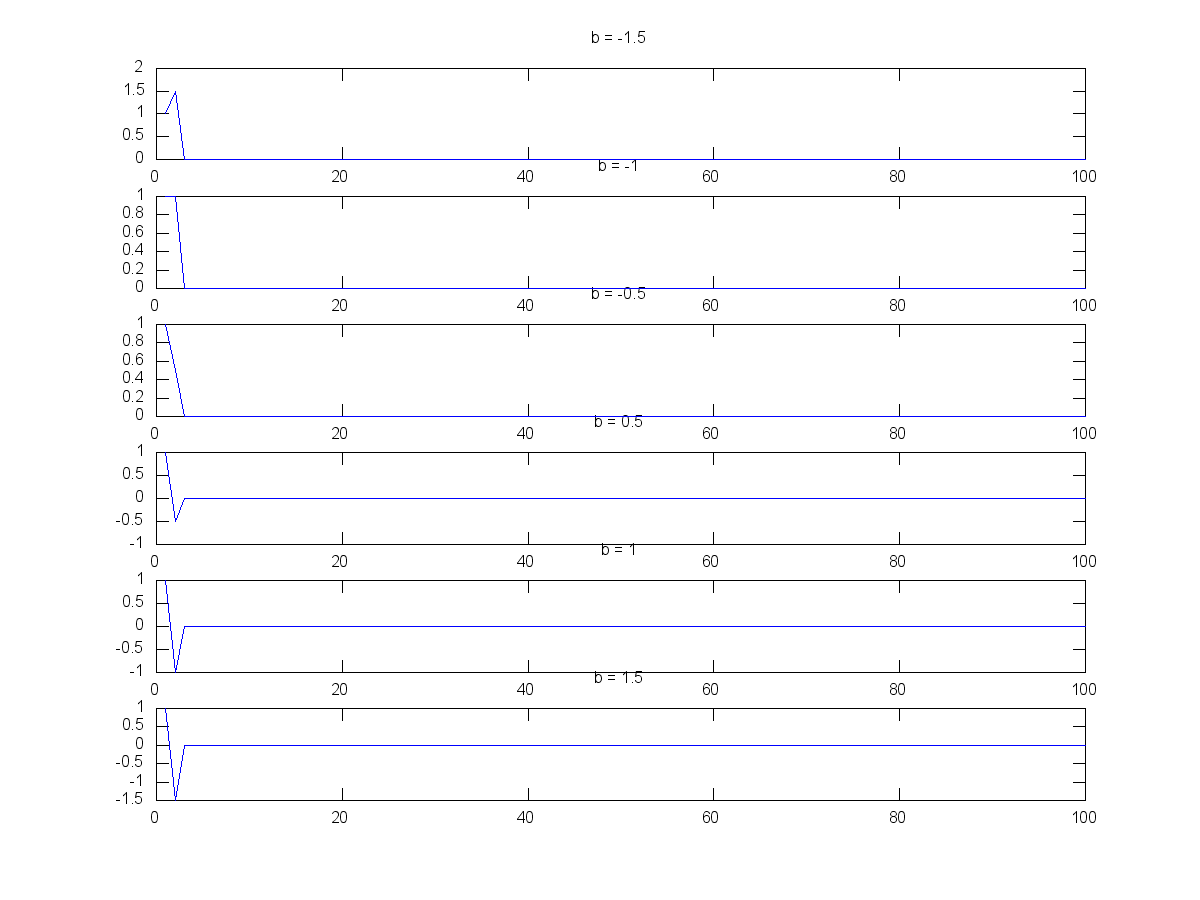
\includegraphics[scale=.3]{out/fig1.png}
      \caption{\label{fig1} Wpływ położenia rzeczywistego zera na odpowiedź impulsową}
      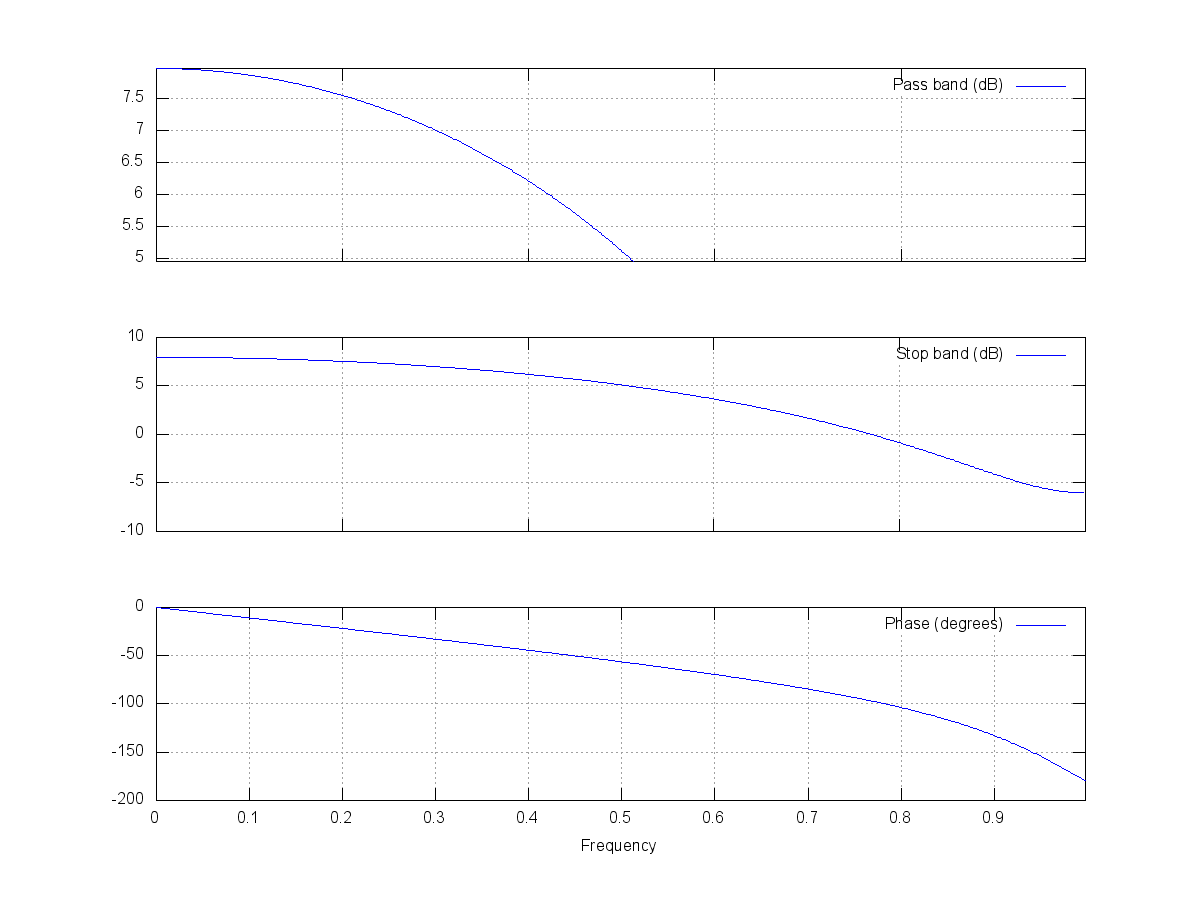
\includegraphics[scale=.3]{out/fig2.png}
      \caption{\label{fig2} Charakterystyka filtru, $b=-1.5$}

    \end{center}
  \end{figure}

  \begin{figure}[htbp]
    \begin{center}
      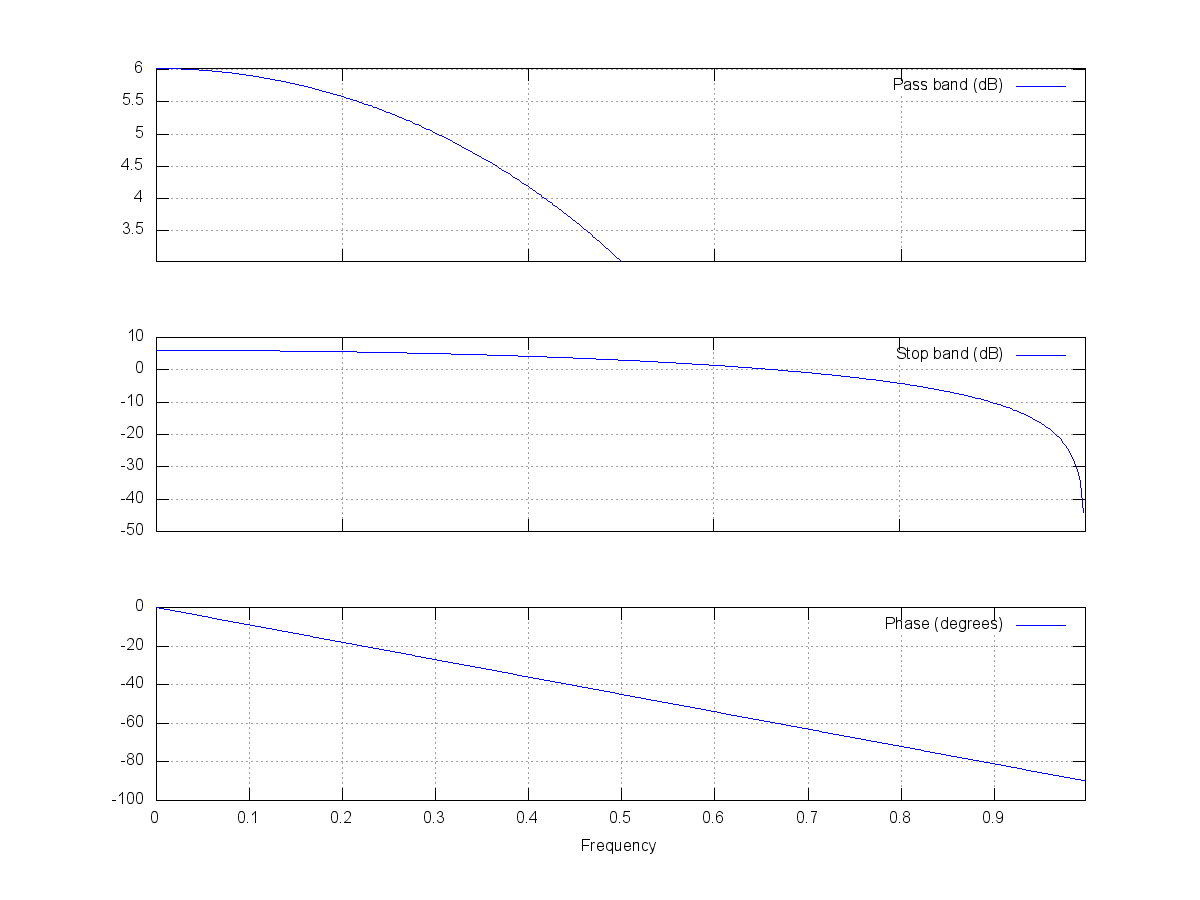
\includegraphics[scale=.3]{out/fig3.png}
      \caption{\label{fig3} Charakterystyka filtru, $b=-1.0$}
      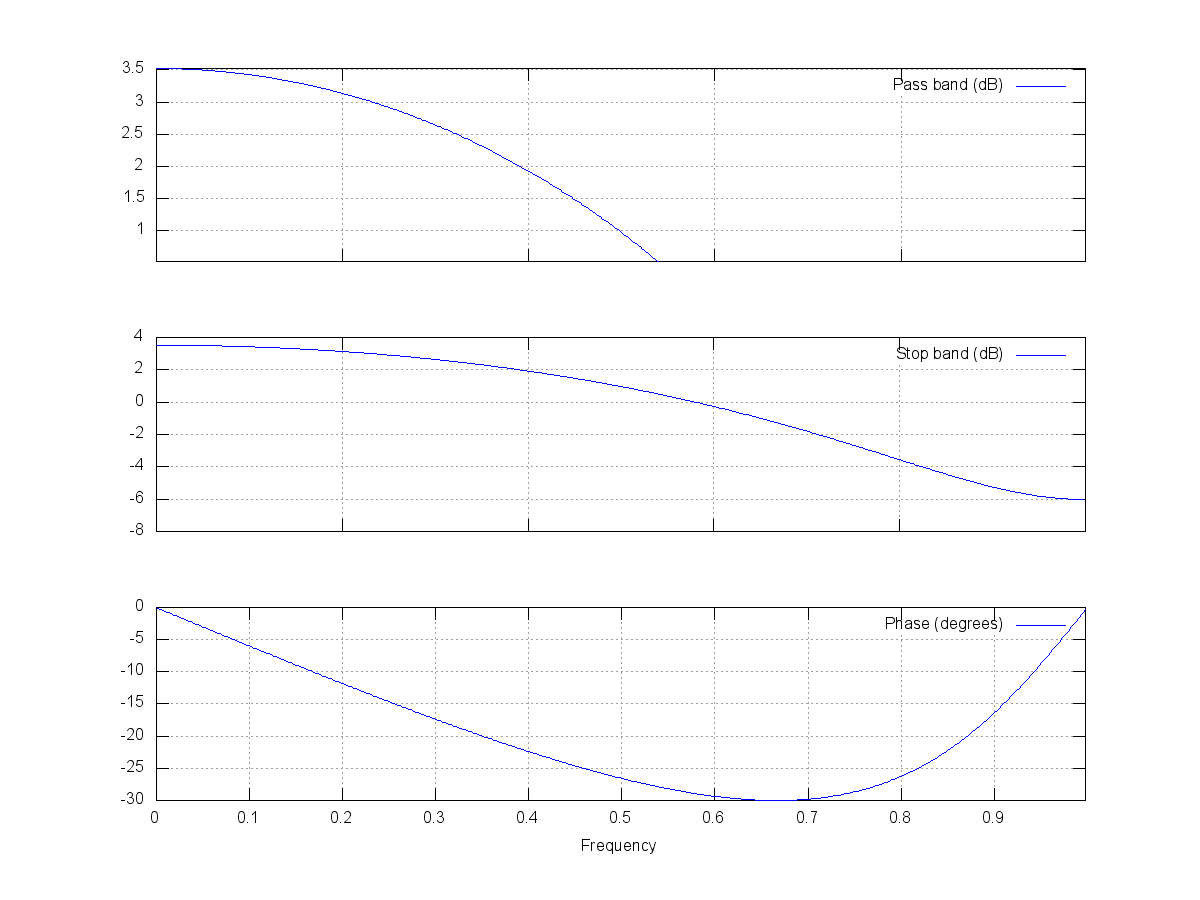
\includegraphics[scale=.3]{out/fig4.png}
      \caption{\label{fig4} Charakterystyka filtru, $b=-0.5$}

    \end{center}
  \end{figure}

  \begin{figure}[htbp]
    \begin{center}
      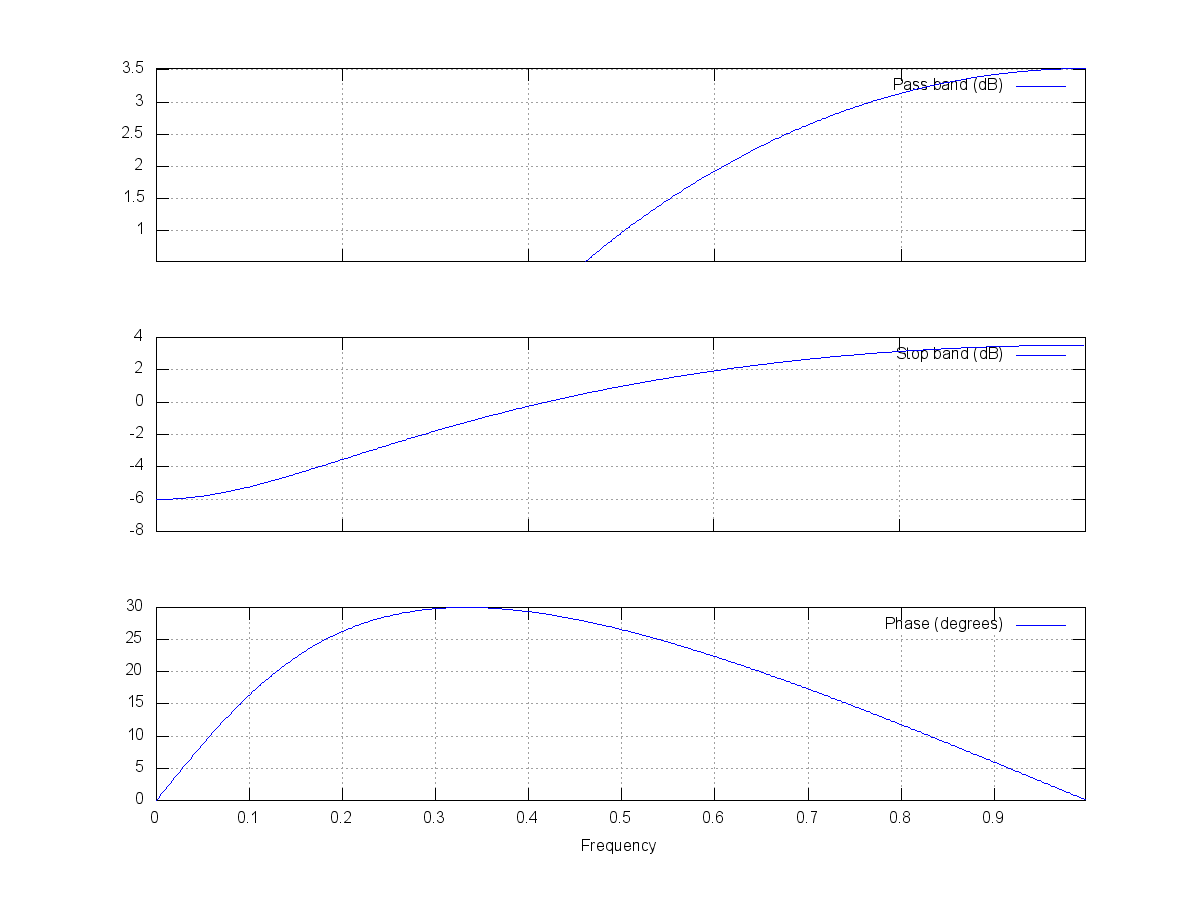
\includegraphics[scale=.3]{out/fig5.png}
      \caption{\label{fig5} Charakterystyka filtru, $b=0.5$}
      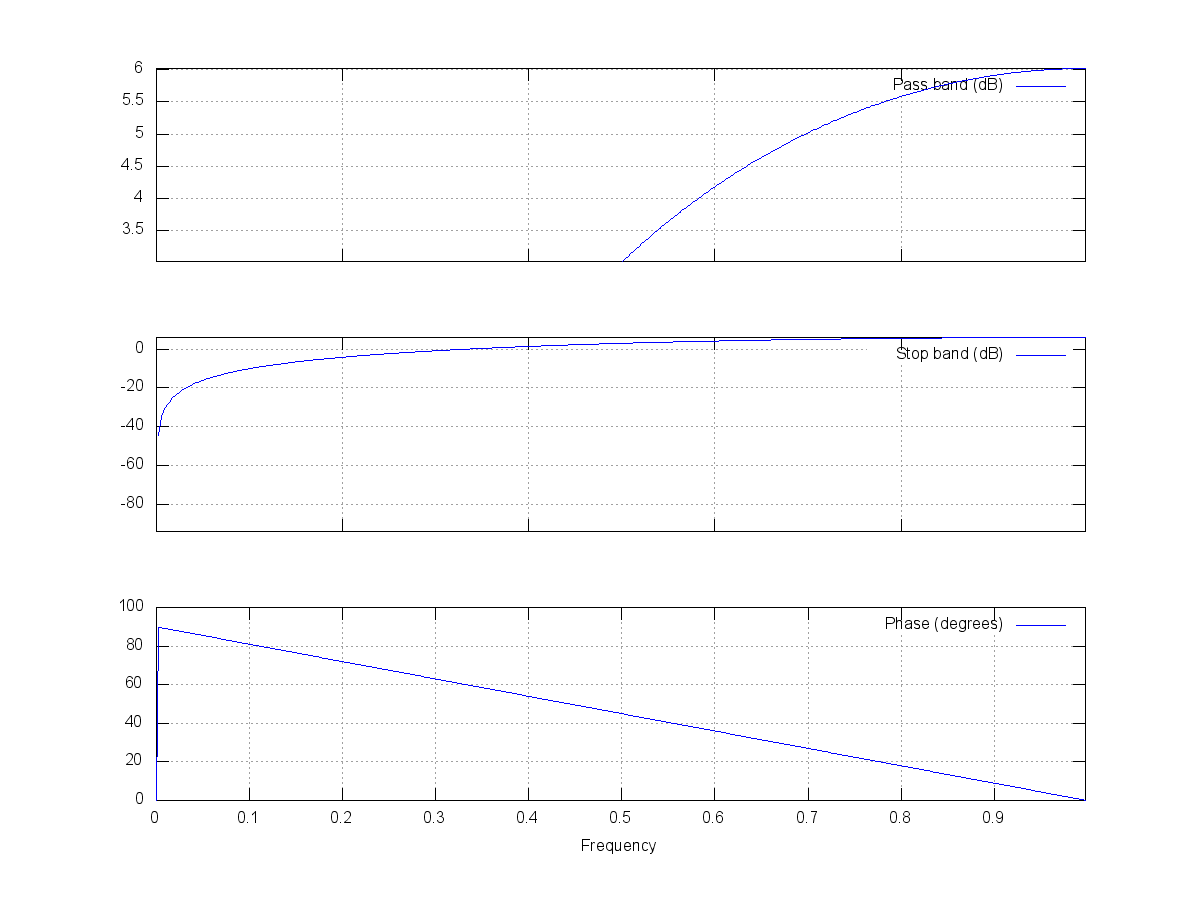
\includegraphics[scale=.3]{out/fig6.png}
      \caption{\label{fig6} Charakterystyka filtru, $b=1.0$}

    \end{center}
  \end{figure}

  \begin{figure}[htbp]
    \begin{center}
      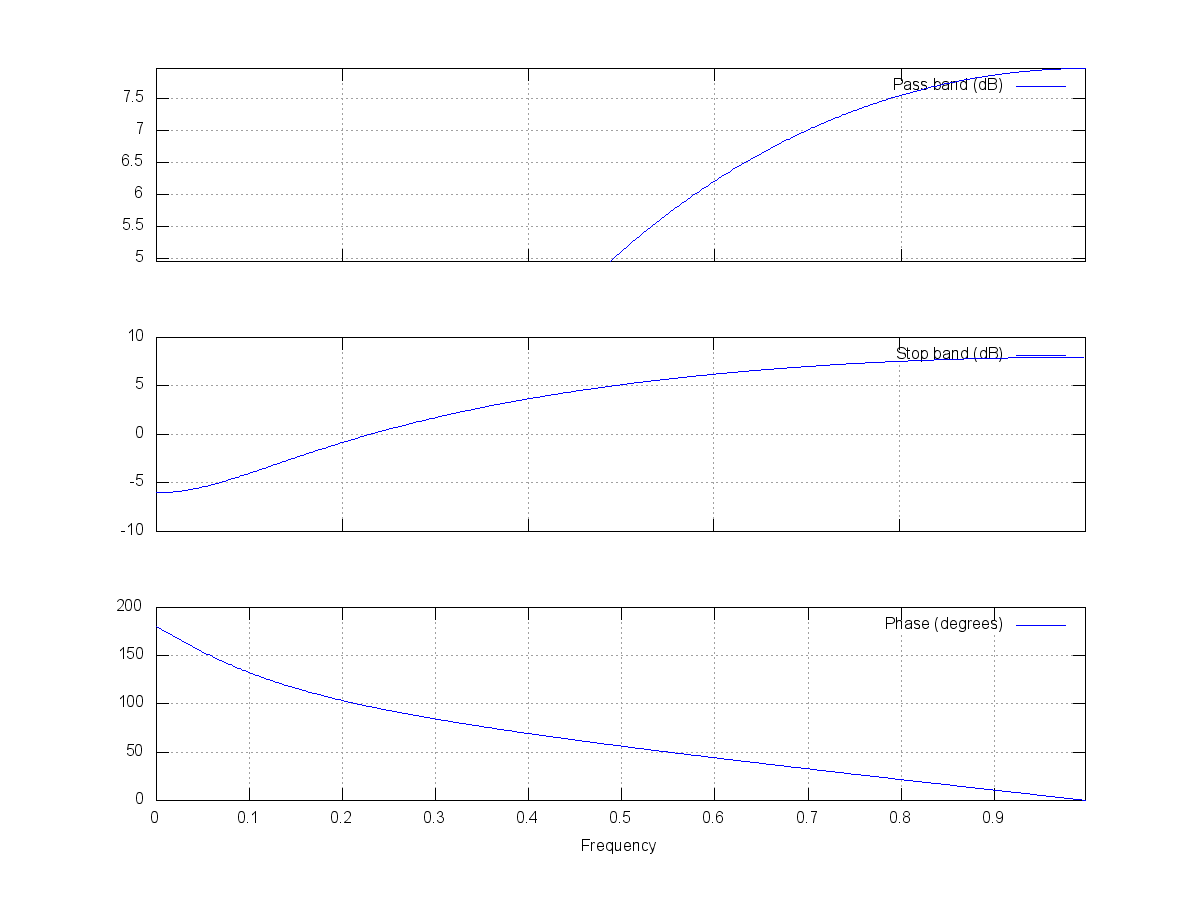
\includegraphics[scale=.3]{out/fig7.png}
      \caption{\label{fig7} Charakterystyka filtru, $b=1.5$}
      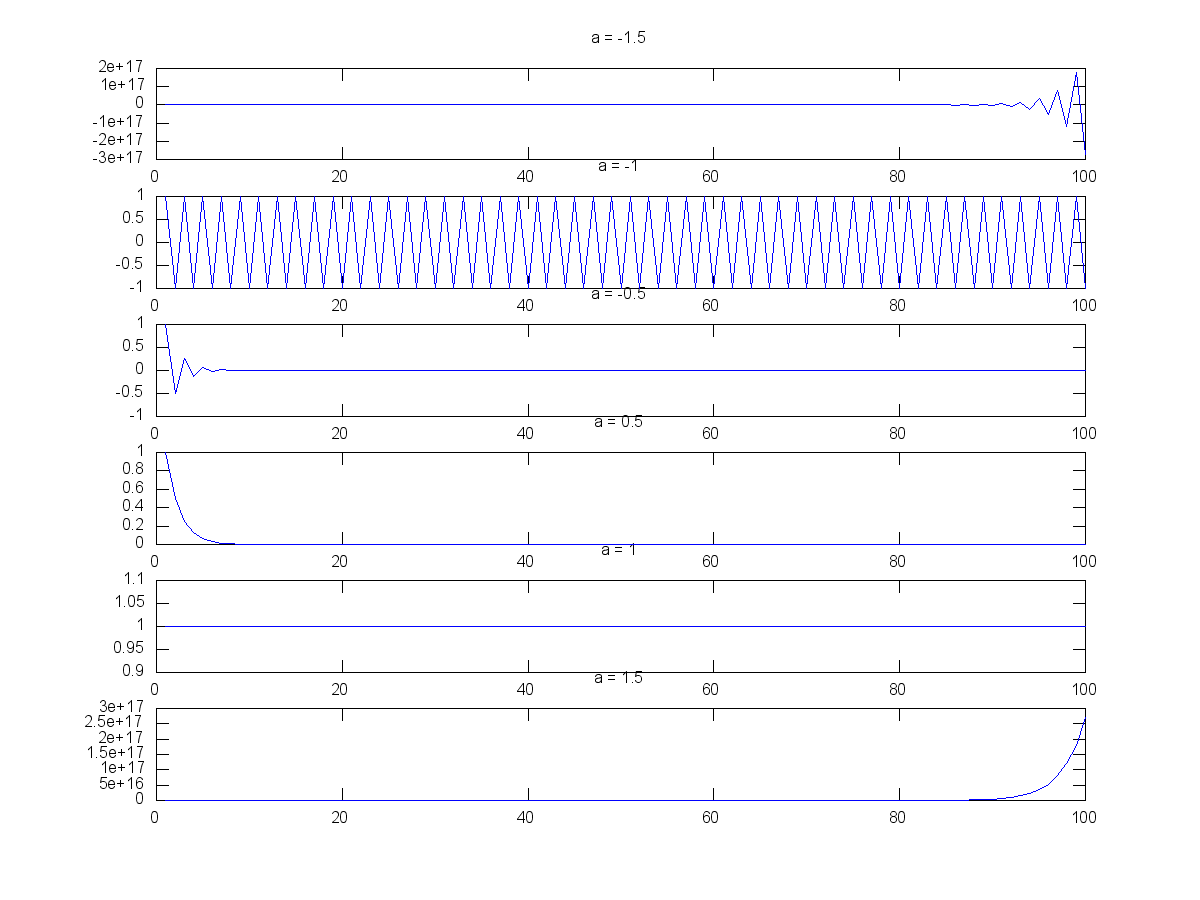
\includegraphics[scale=.3]{out/fig8.png}
      \caption{\label{fig8} Wpływ położenia rzeczywistego bieguna na odpowiedź impulsową}

    \end{center}
  \end{figure}

  \begin{figure}[htbp]
    \begin{center}
      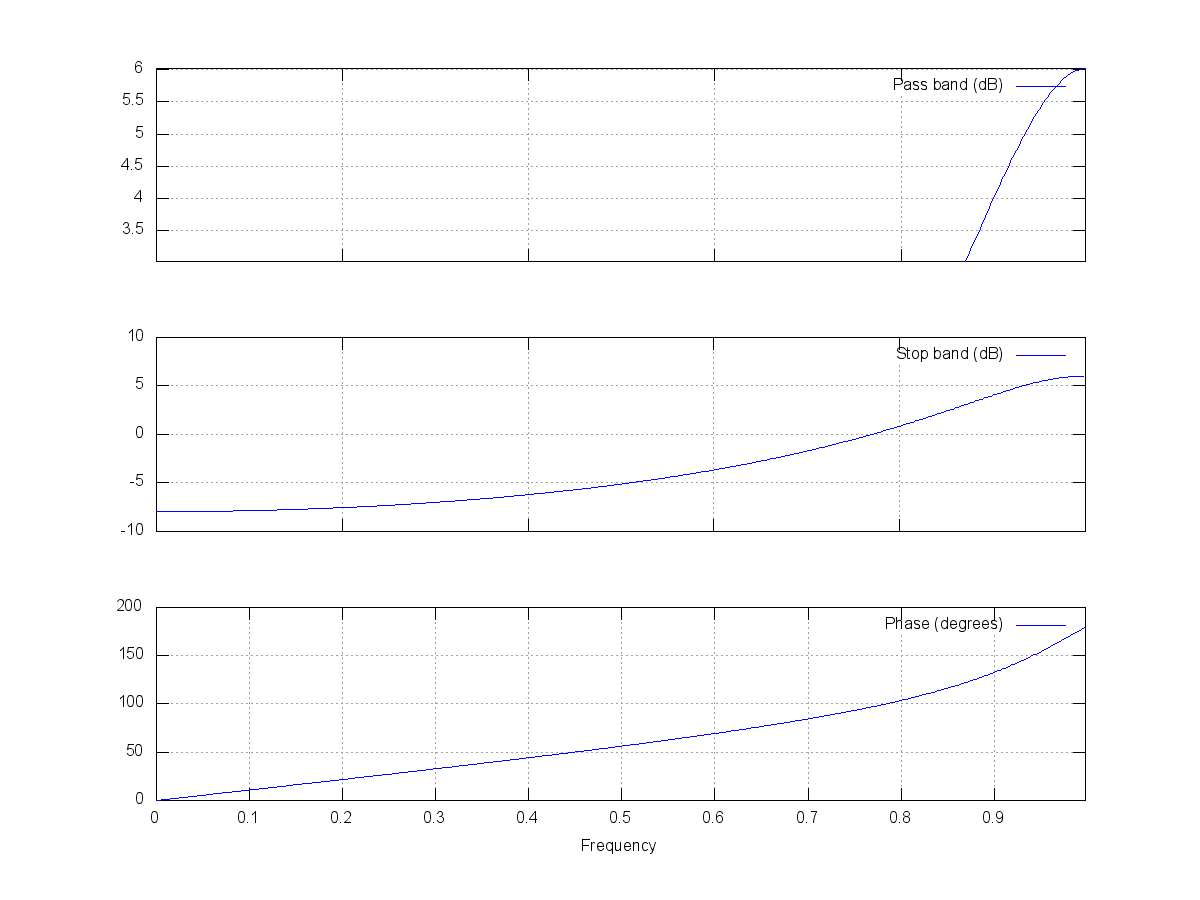
\includegraphics[scale=.3]{out/fig9.png}
      \caption{\label{fig9} Charakterystyka filtru, $a=-1.5$}
      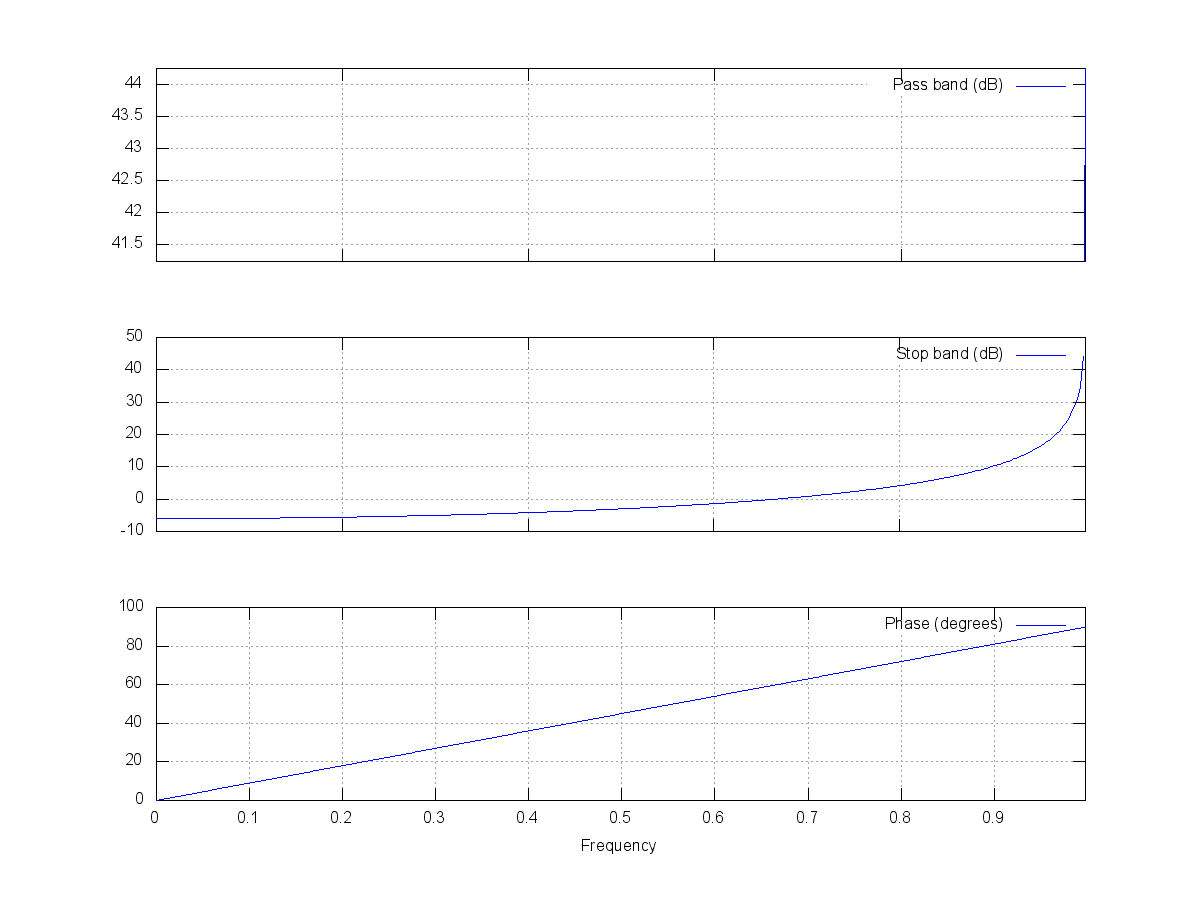
\includegraphics[scale=.3]{out/fig10.png}
      \caption{\label{fig10} Charakterystyka filtru, $a=-1.0$}

    \end{center}
  \end{figure}

  \begin{figure}[htbp]
    \begin{center}
      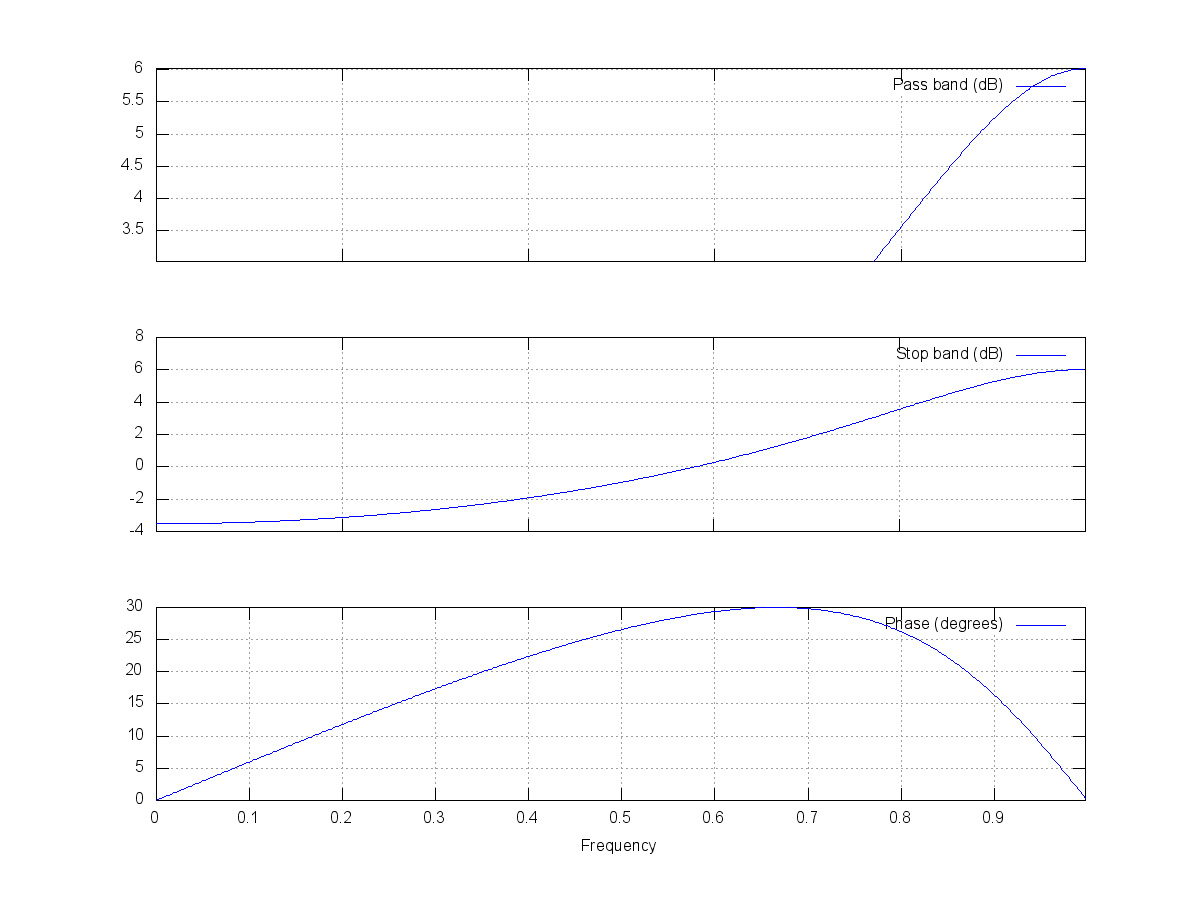
\includegraphics[scale=.3]{out/fig11.png}
      \caption{\label{fig11} Charakterystyka filtru, $a=-0.5$}
      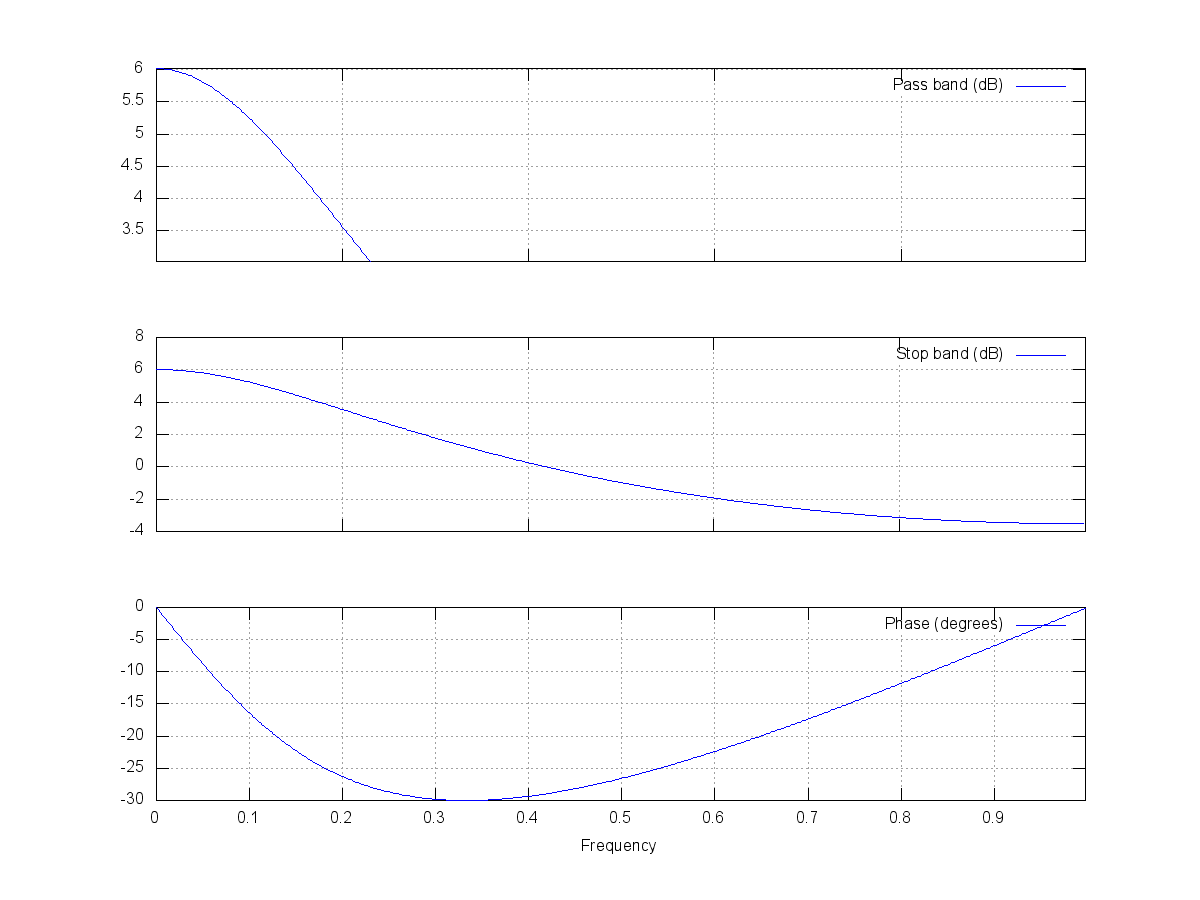
\includegraphics[scale=.3]{out/fig12.png}
      \caption{\label{fig12} Charakterystyka filtru, $a=0.5$}

    \end{center}
  \end{figure}

  \begin{figure}[htbp]
    \begin{center}
      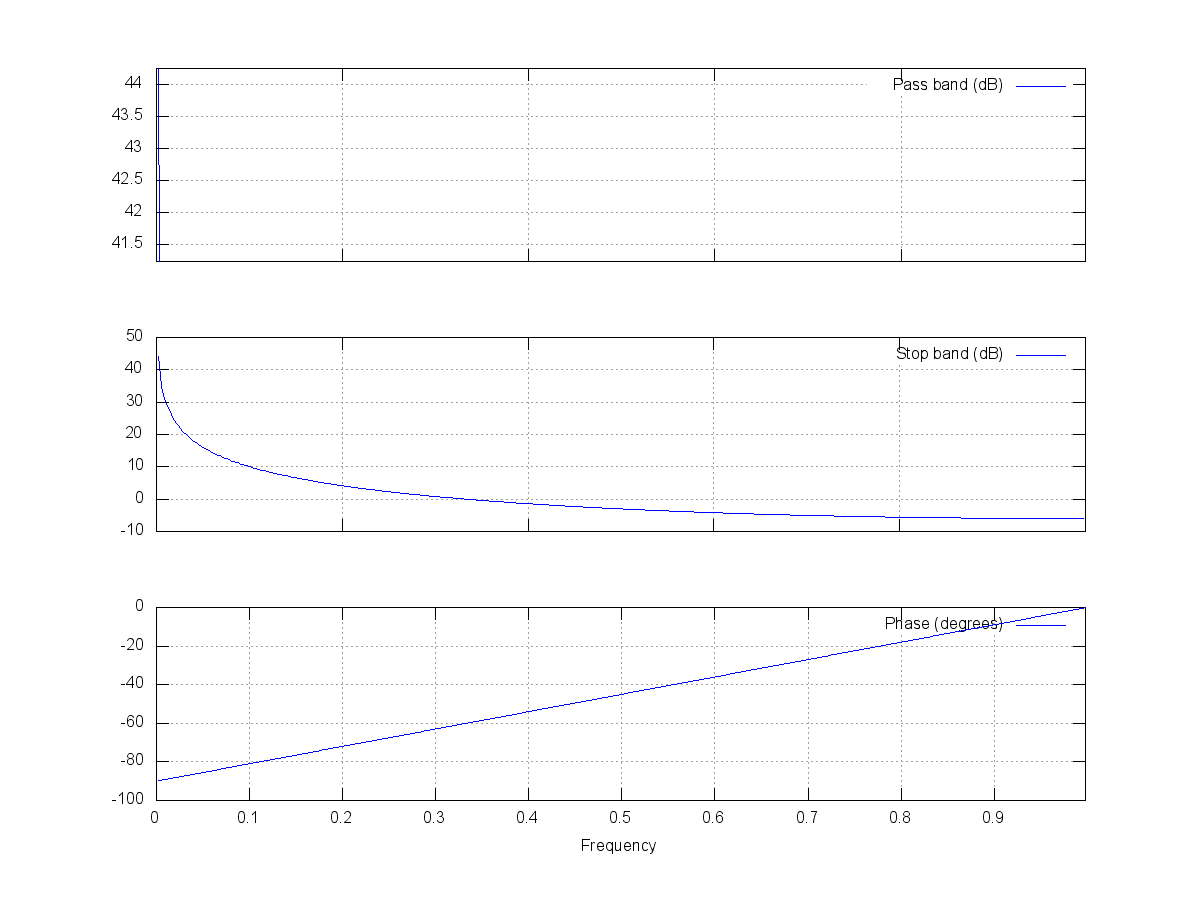
\includegraphics[scale=.3]{out/fig13.png}
      \caption{\label{fig13} Charakterystyka filtru, $a=1.0$}
      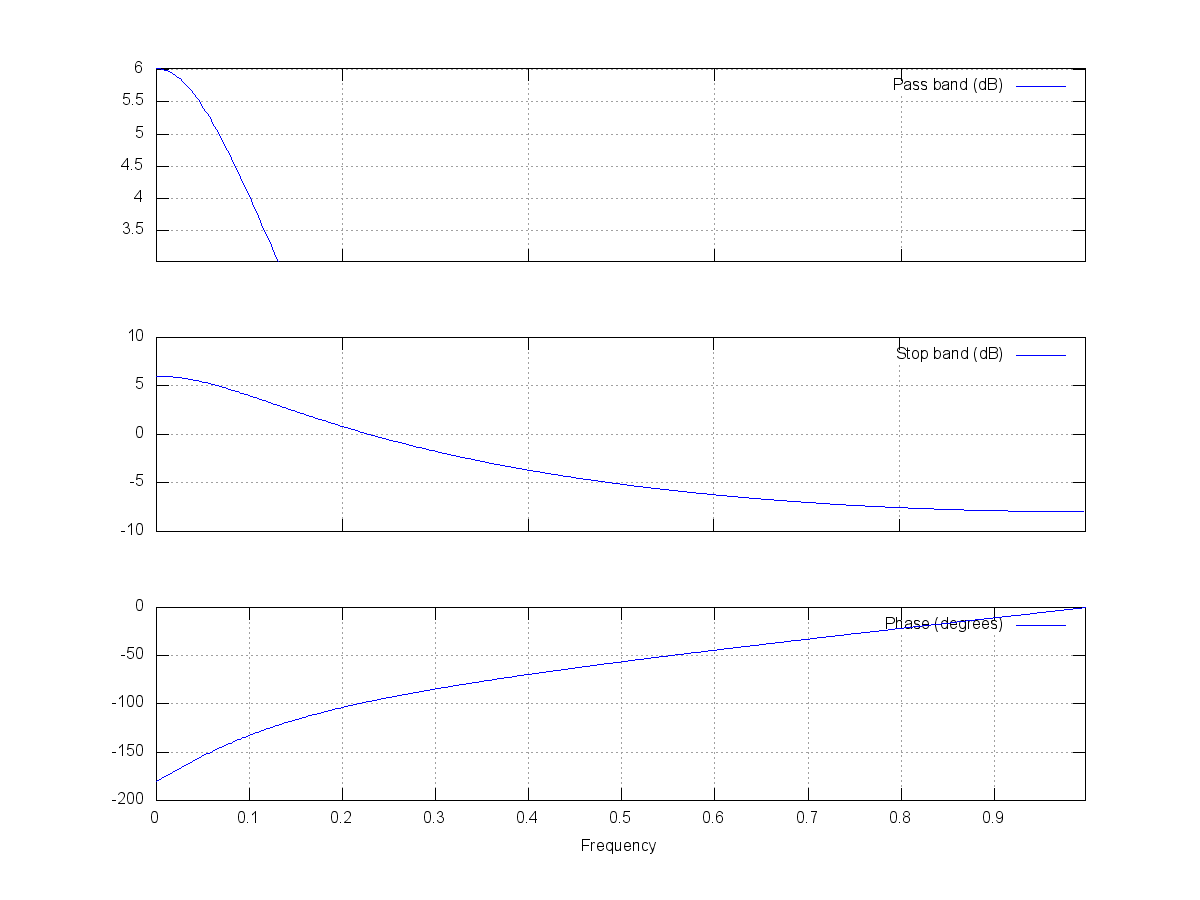
\includegraphics[scale=.3]{out/fig14.png}
      \caption{\label{fig14} Charakterystyka filtru, $a=1.5$}

    \end{center}
  \end{figure}

  \begin{figure}[htbp]
    \begin{center}
      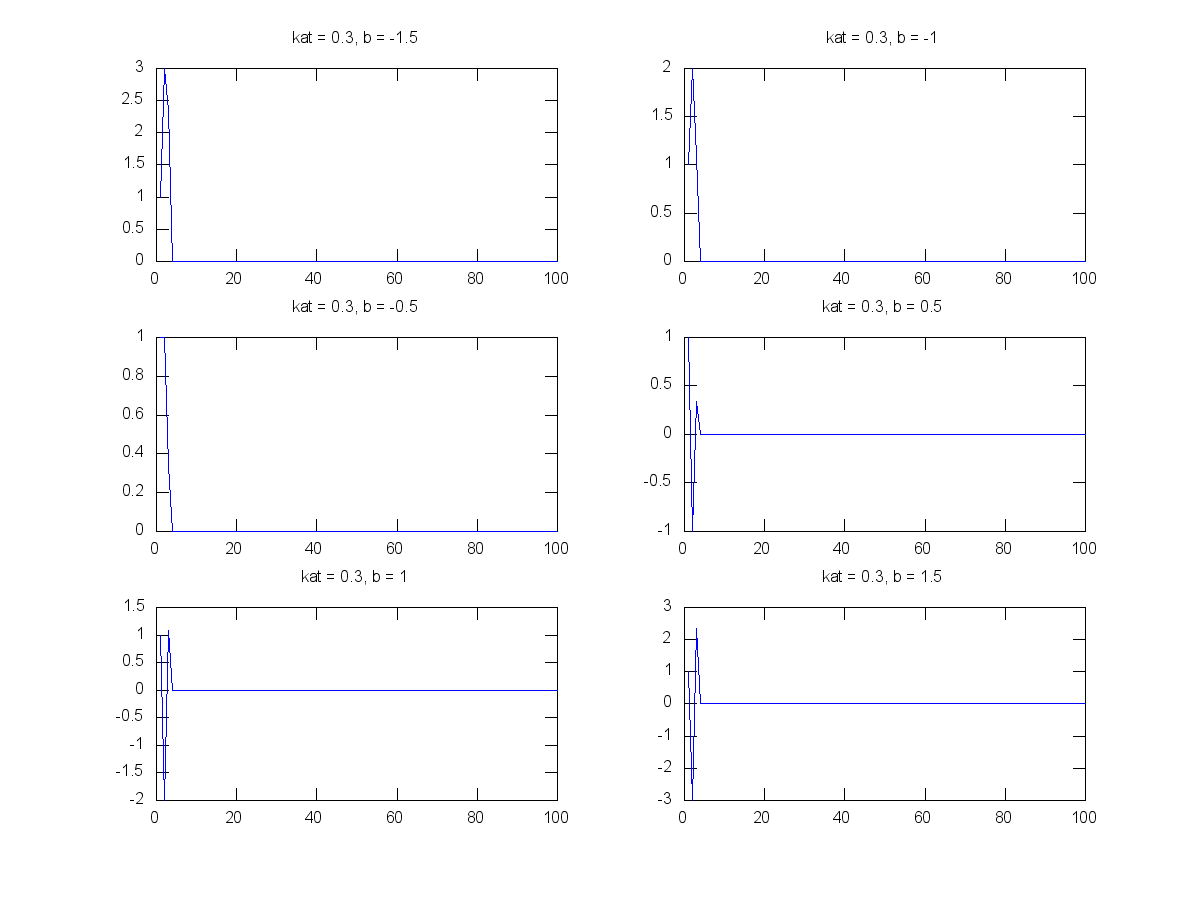
\includegraphics[scale=.3]{out/fig15.png}
      \caption{\label{fig15} Wpływ położenia zespolonego zera na odpowiedź impulsową (cz. 1)}
      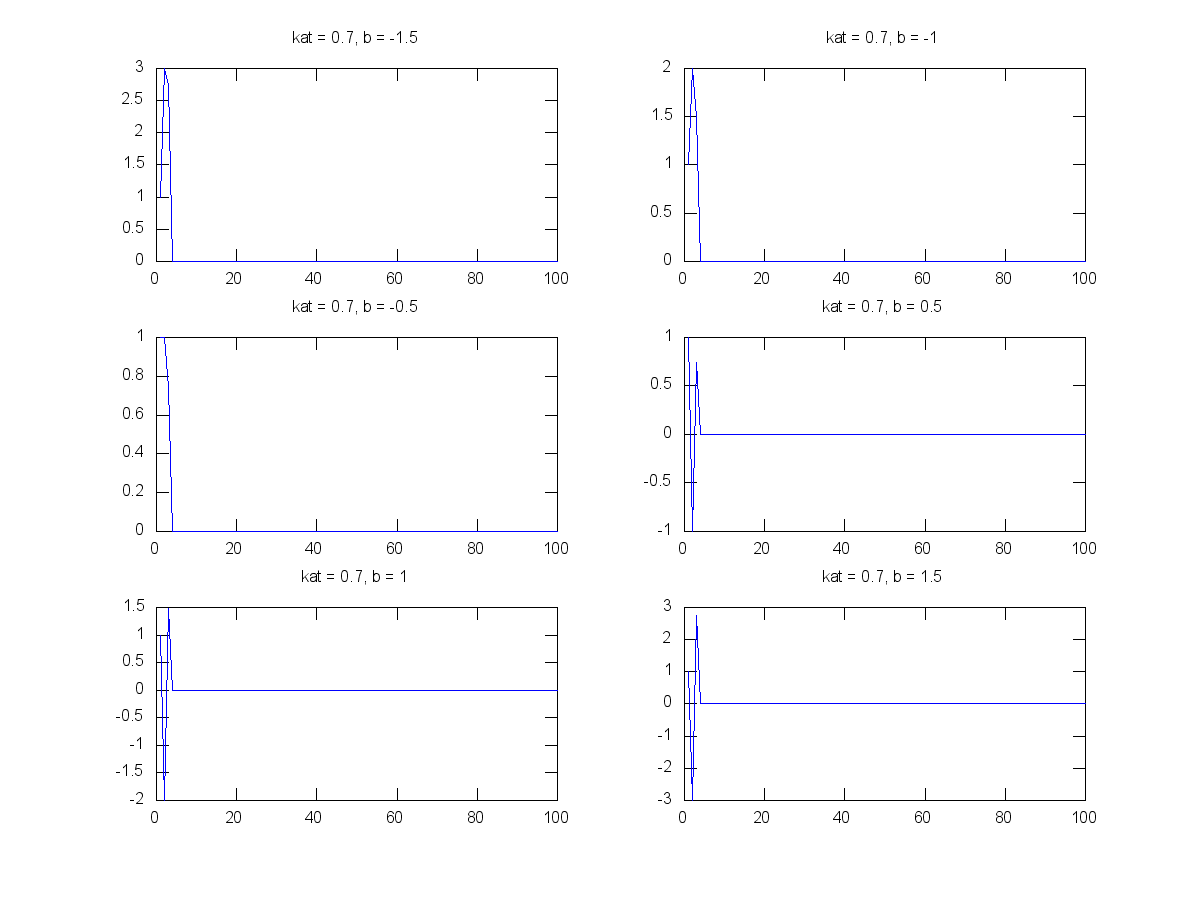
\includegraphics[scale=.3]{out/fig16.png}
      \caption{\label{fig16} Wpływ położenia zespolonego zera na odpowiedź impulsową (cz. 2)}

    \end{center}
  \end{figure}

  \begin{figure}[htbp]
    \begin{center}
      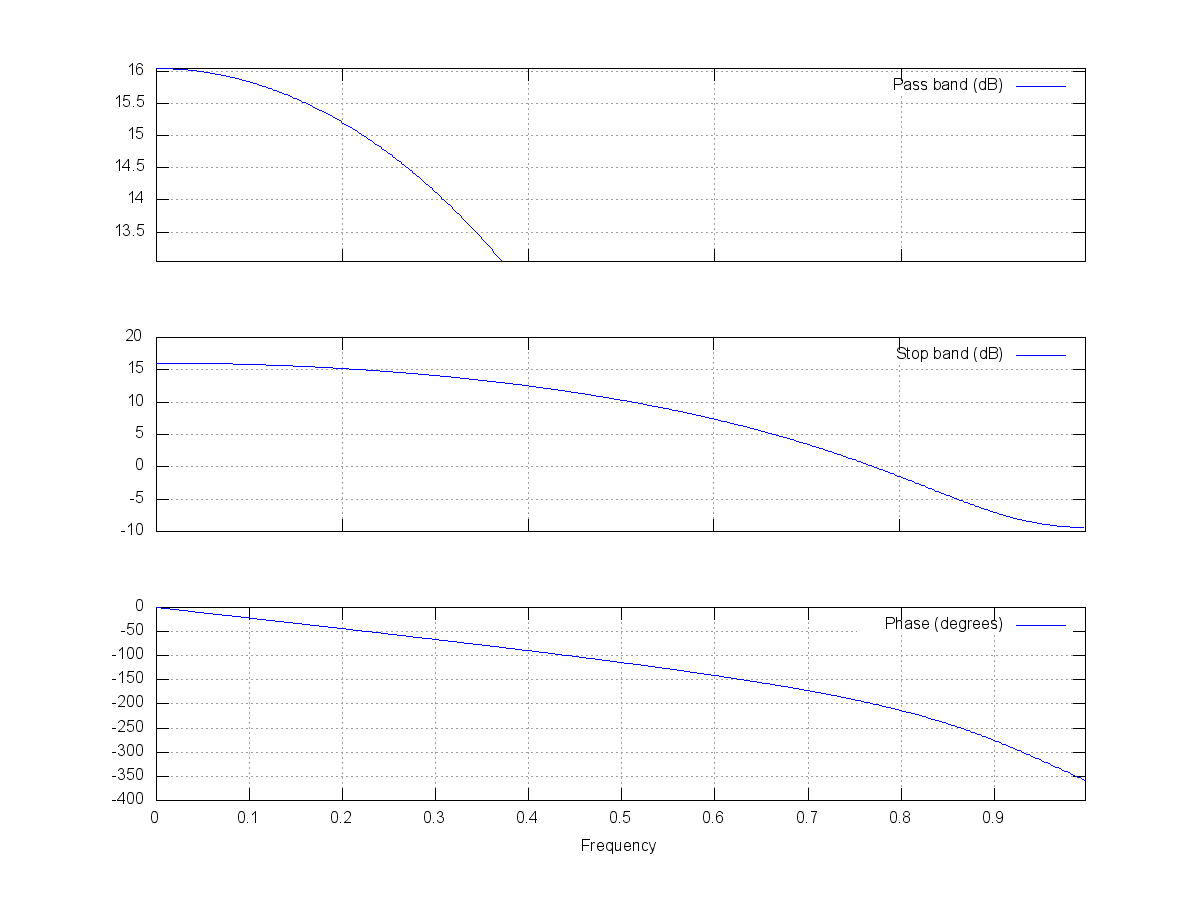
\includegraphics[scale=.3]{out/fig17.png}
      \caption{\label{fig17} Charakterystyka filtru, $b=-1.5\pm0.3i$}
      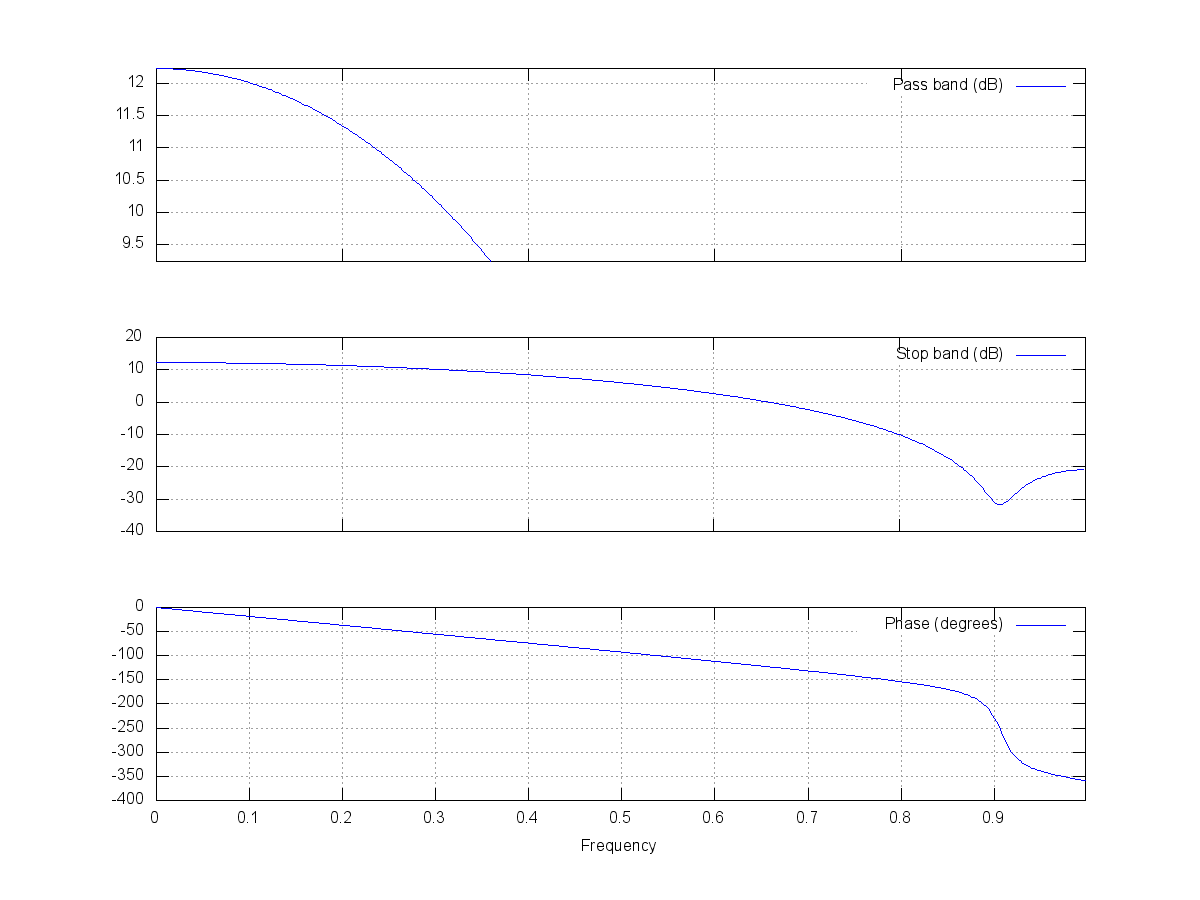
\includegraphics[scale=.3]{out/fig18.png}
      \caption{\label{fig18} Charakterystyka filtru, $b=-1.0\pm0.3i$}

    \end{center}
  \end{figure}

  \begin{figure}[htbp]
    \begin{center}
      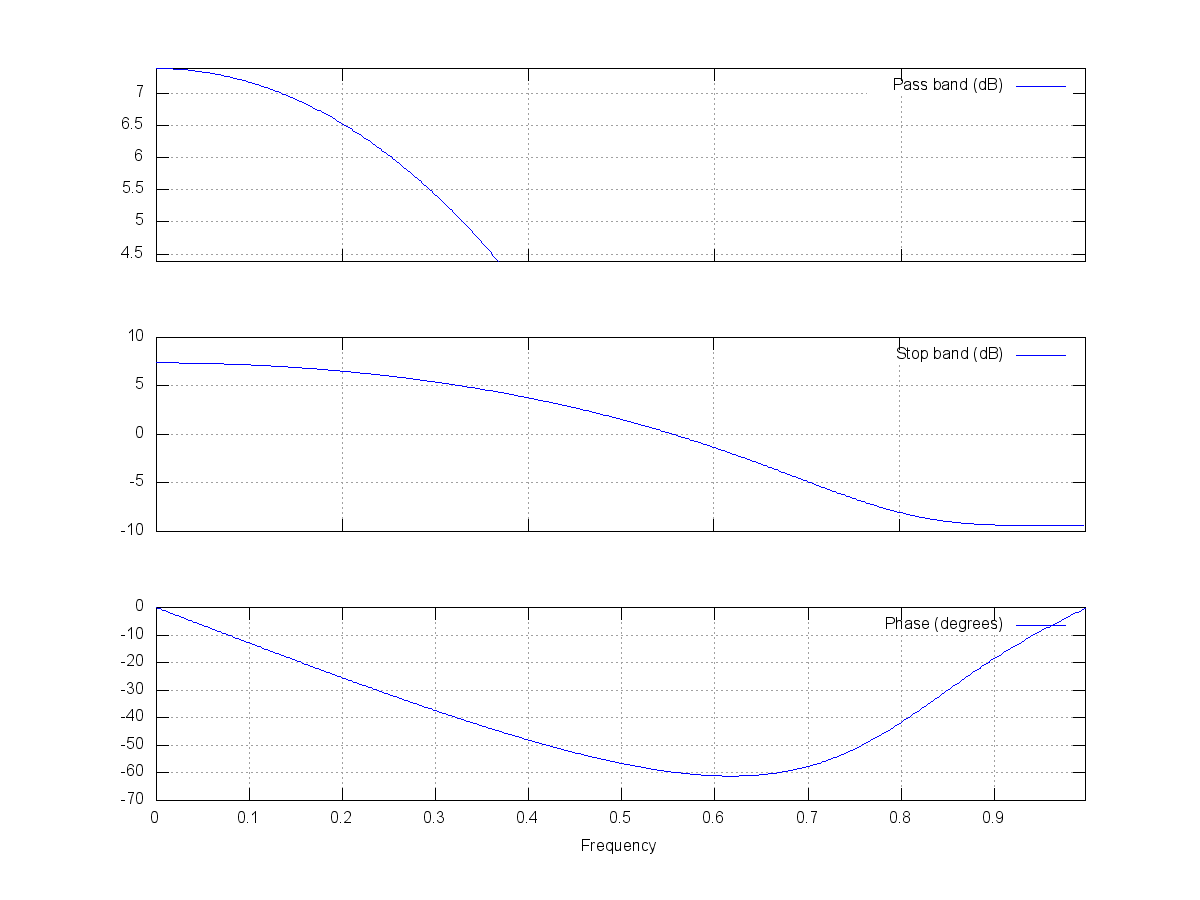
\includegraphics[scale=.3]{out/fig19.png}
      \caption{\label{fig19} Charakterystyka filtru, $b=-0.5\pm0.3i$}
      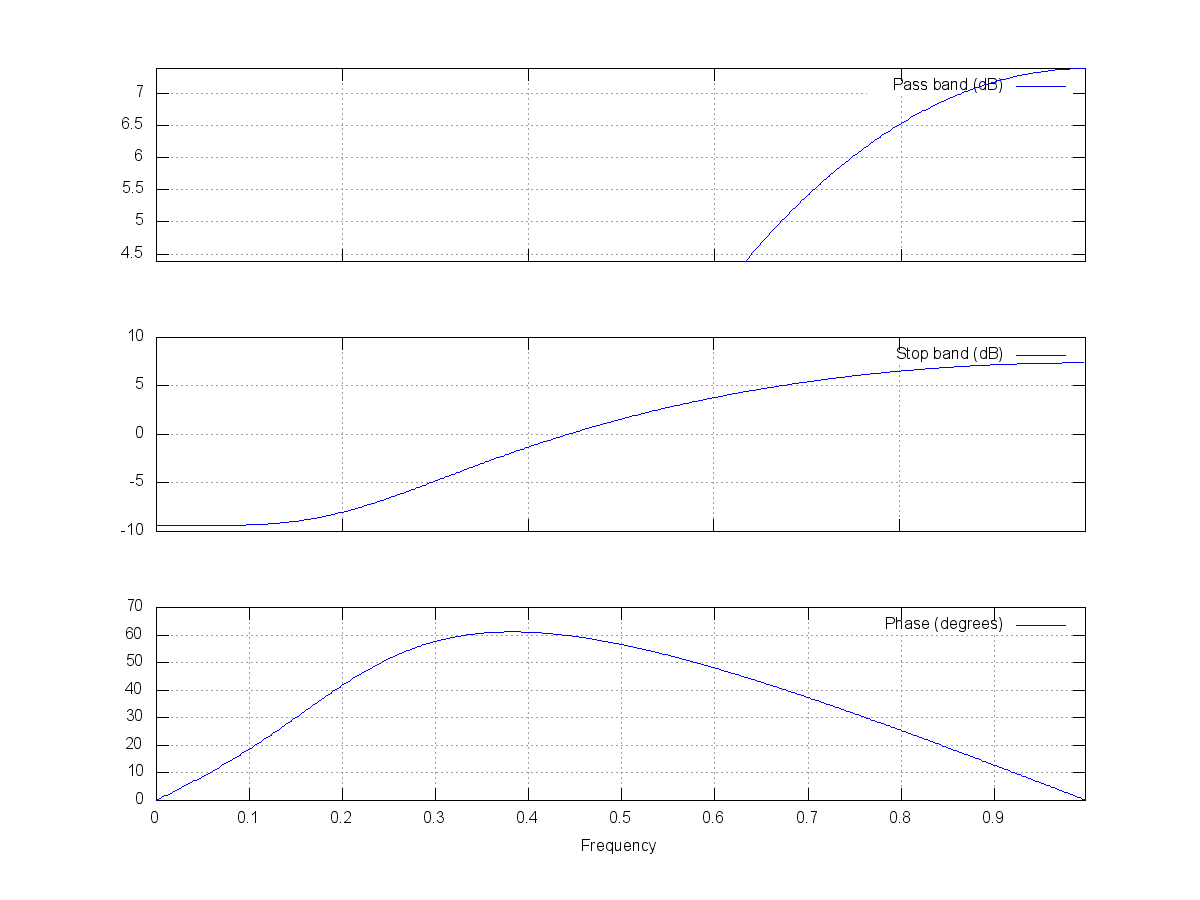
\includegraphics[scale=.3]{out/fig20.png}
      \caption{\label{fig20} Charakterystyka filtru, $b=0.5\pm0.3i$}

    \end{center}
  \end{figure}

  \begin{figure}[htbp]
    \begin{center}
      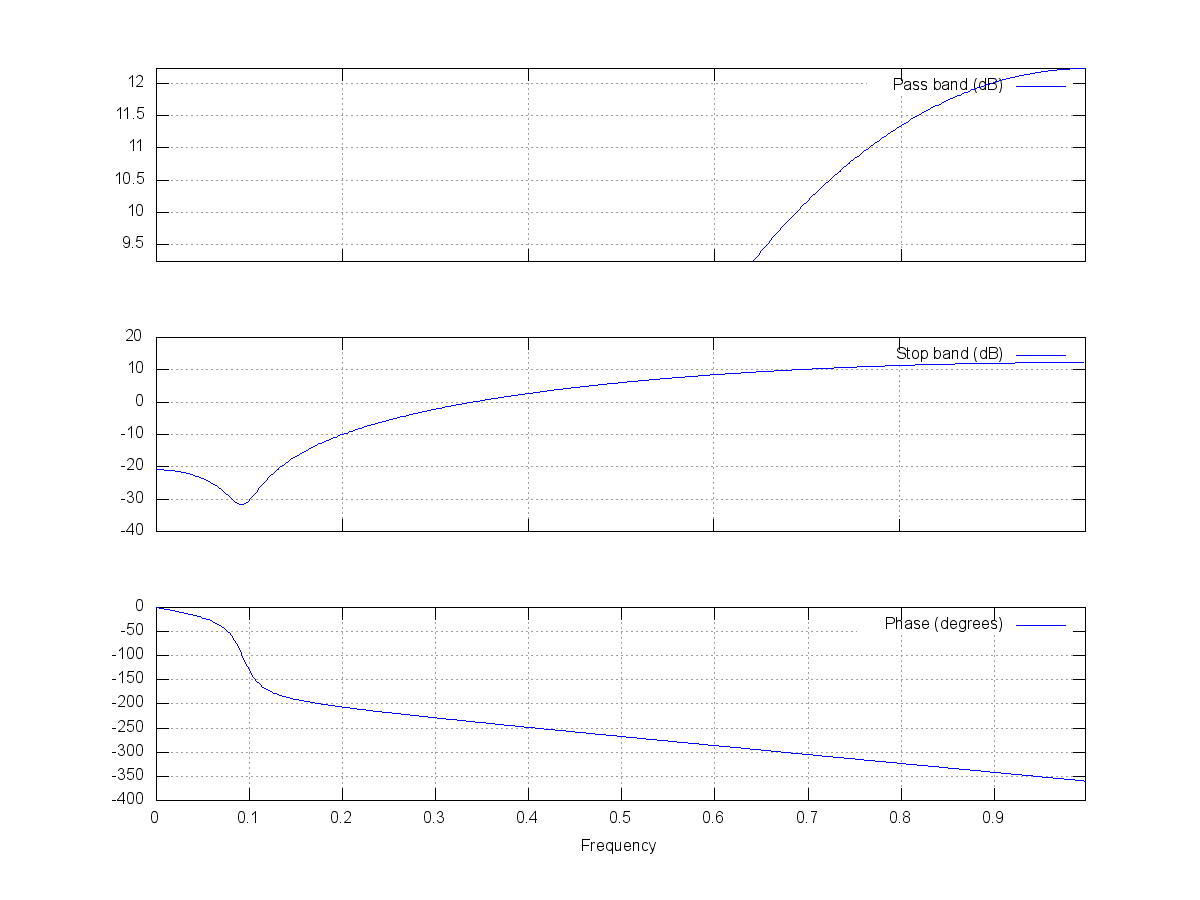
\includegraphics[scale=.3]{out/fig21.png}
      \caption{\label{fig21} Charakterystyka filtru, $b=1.0\pm0.3i$}
      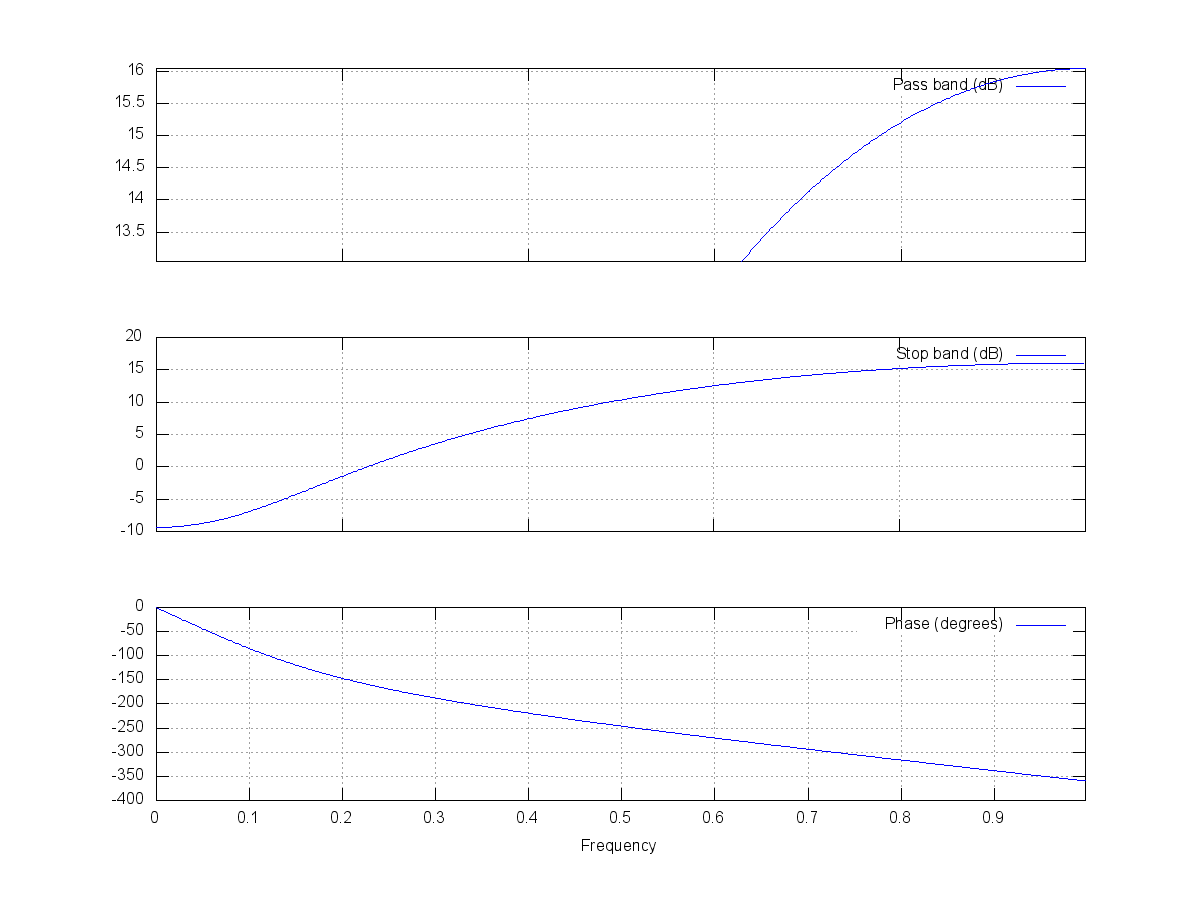
\includegraphics[scale=.3]{out/fig22.png}
      \caption{\label{fig22} Charakterystyka filtru, $b=1.5\pm0.3i$}

    \end{center}
  \end{figure}

  \begin{figure}[htbp]
    \begin{center}
      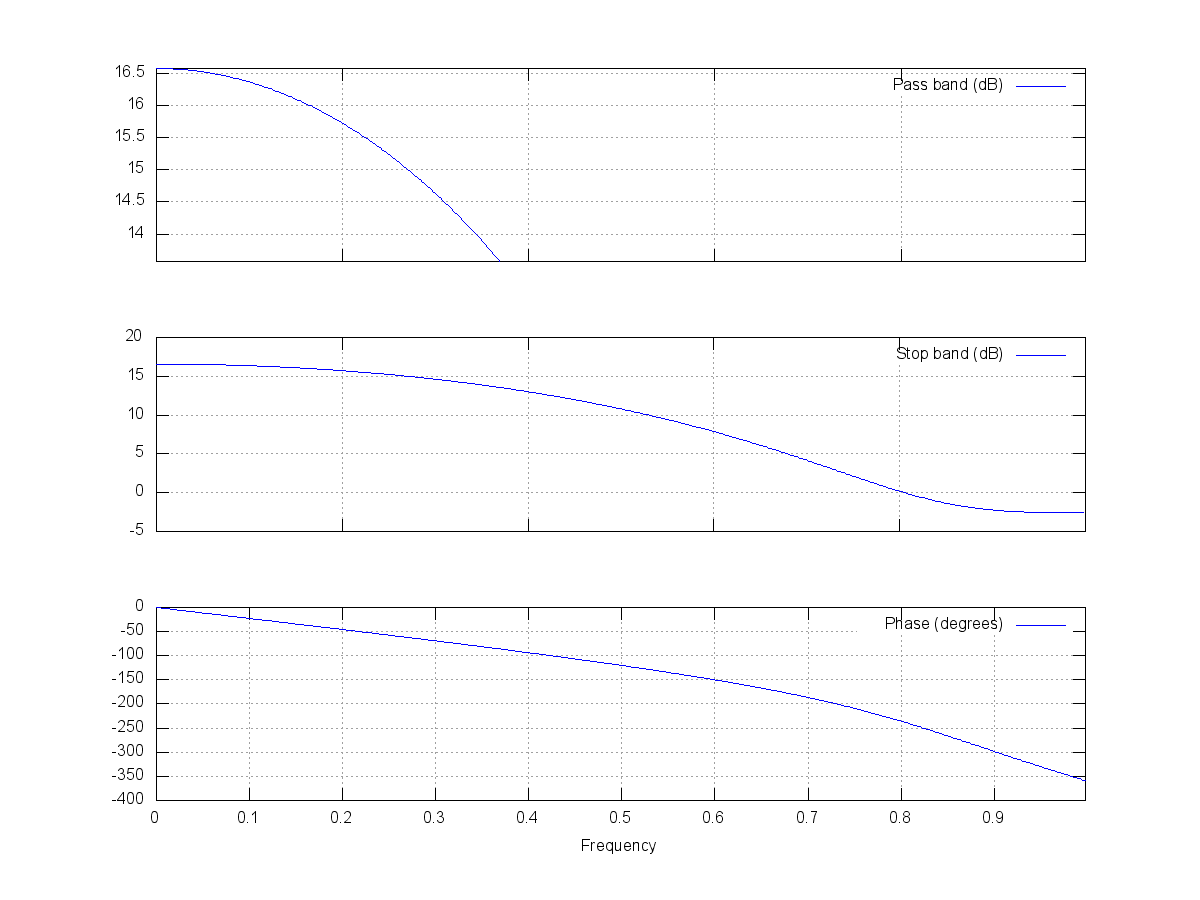
\includegraphics[scale=.3]{out/fig23.png}
      \caption{\label{fig23} Charakterystyka filtru, $b=-1.5\pm0.7i$}
      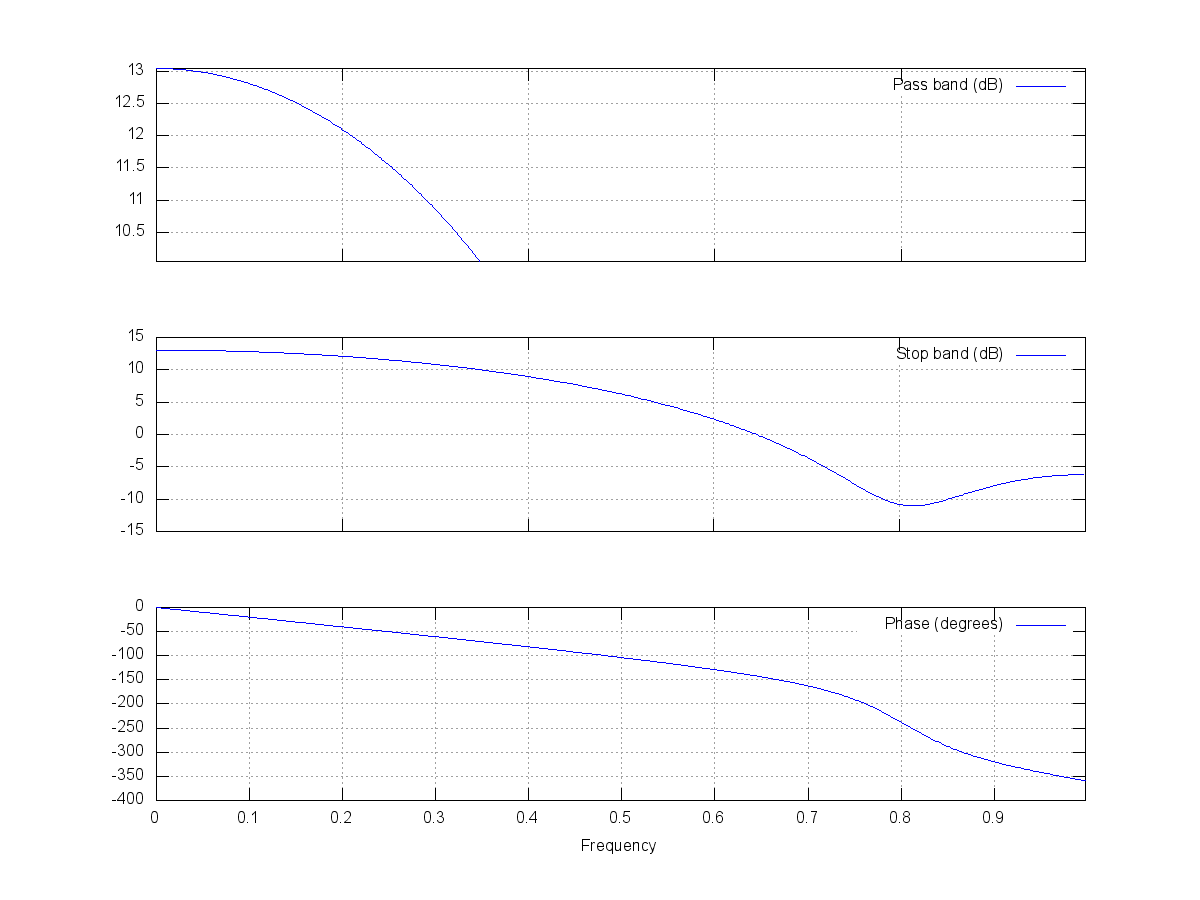
\includegraphics[scale=.3]{out/fig24.png}
      \caption{\label{fig24} Charakterystyka filtru, $b=-1.0\pm0.7i$}

    \end{center}
  \end{figure}

  \begin{figure}[htbp]
    \begin{center}
      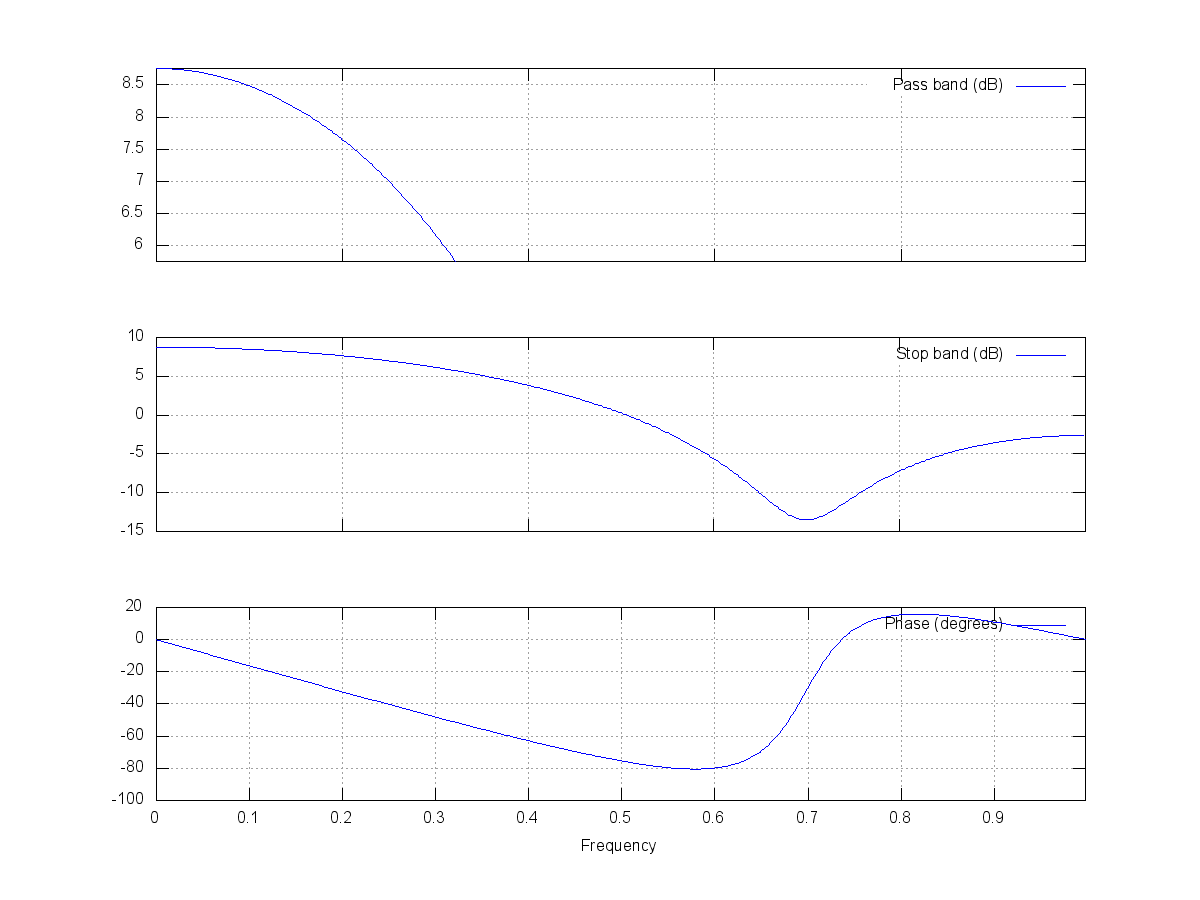
\includegraphics[scale=.3]{out/fig25.png}
      \caption{\label{fig25} Charakterystyka filtru, $b=-0.5\pm0.7i$}
      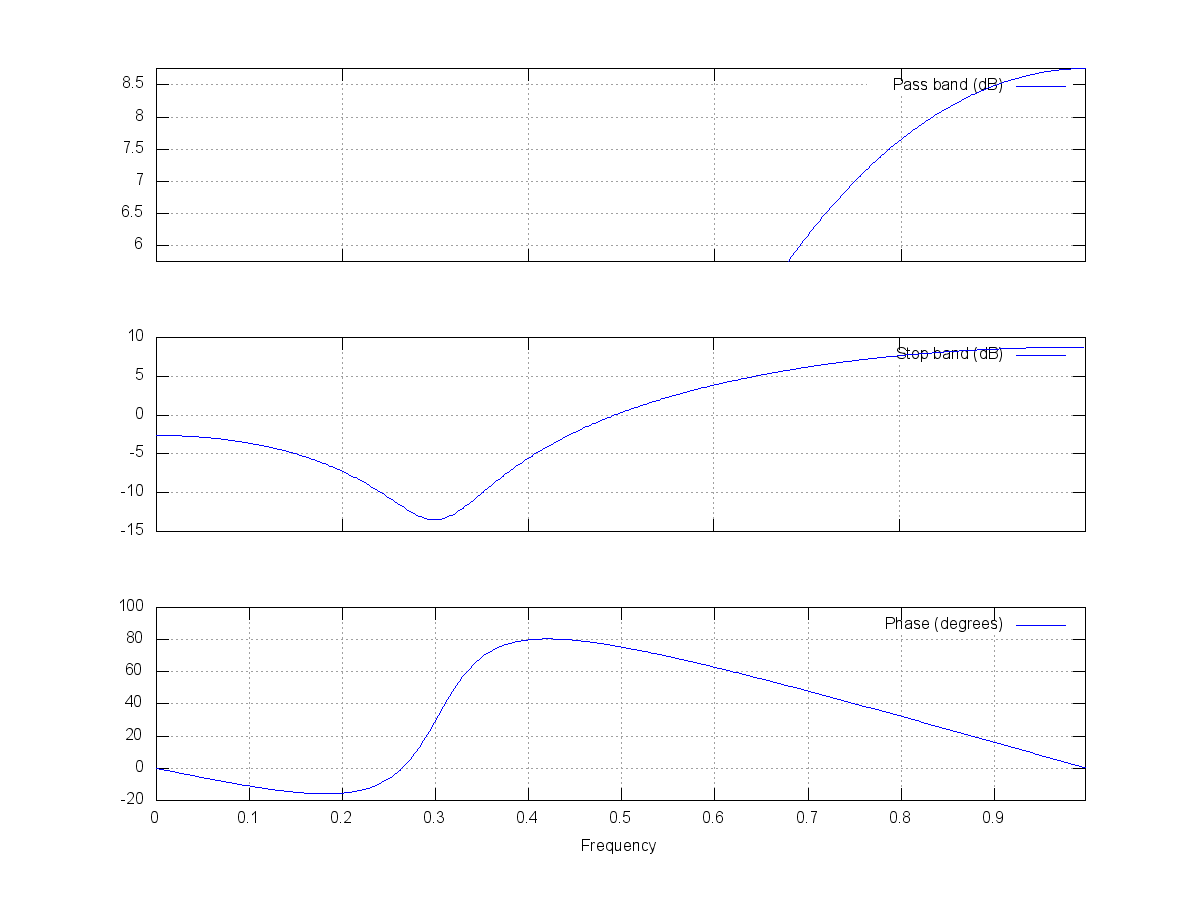
\includegraphics[scale=.3]{out/fig26.png}
      \caption{\label{fig26} Charakterystyka filtru, $b=0.5\pm0.7i$}

    \end{center}
  \end{figure}

  \begin{figure}[htbp]
    \begin{center}
      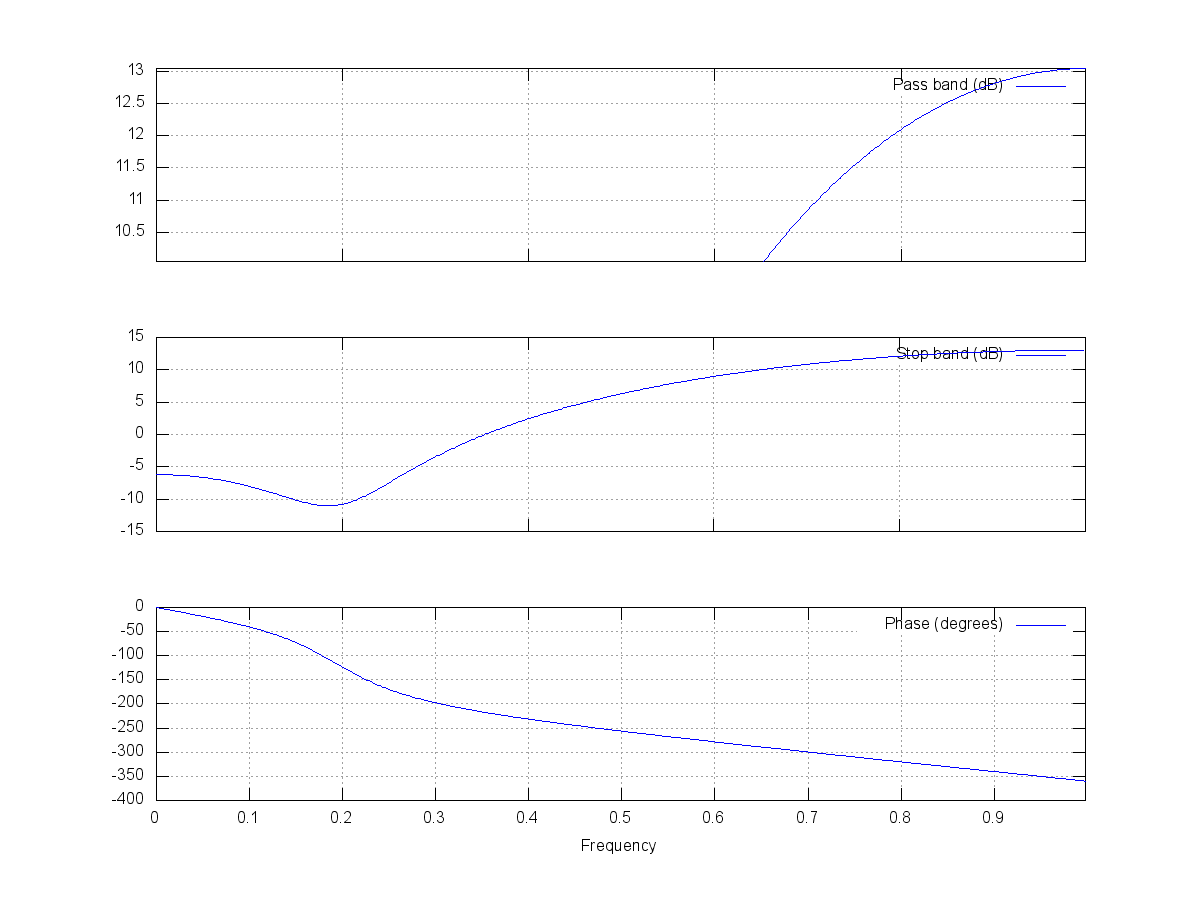
\includegraphics[scale=.3]{out/fig27.png}
      \caption{\label{fig27} Charakterystyka filtru, $b=1.0\pm0.7i$}
      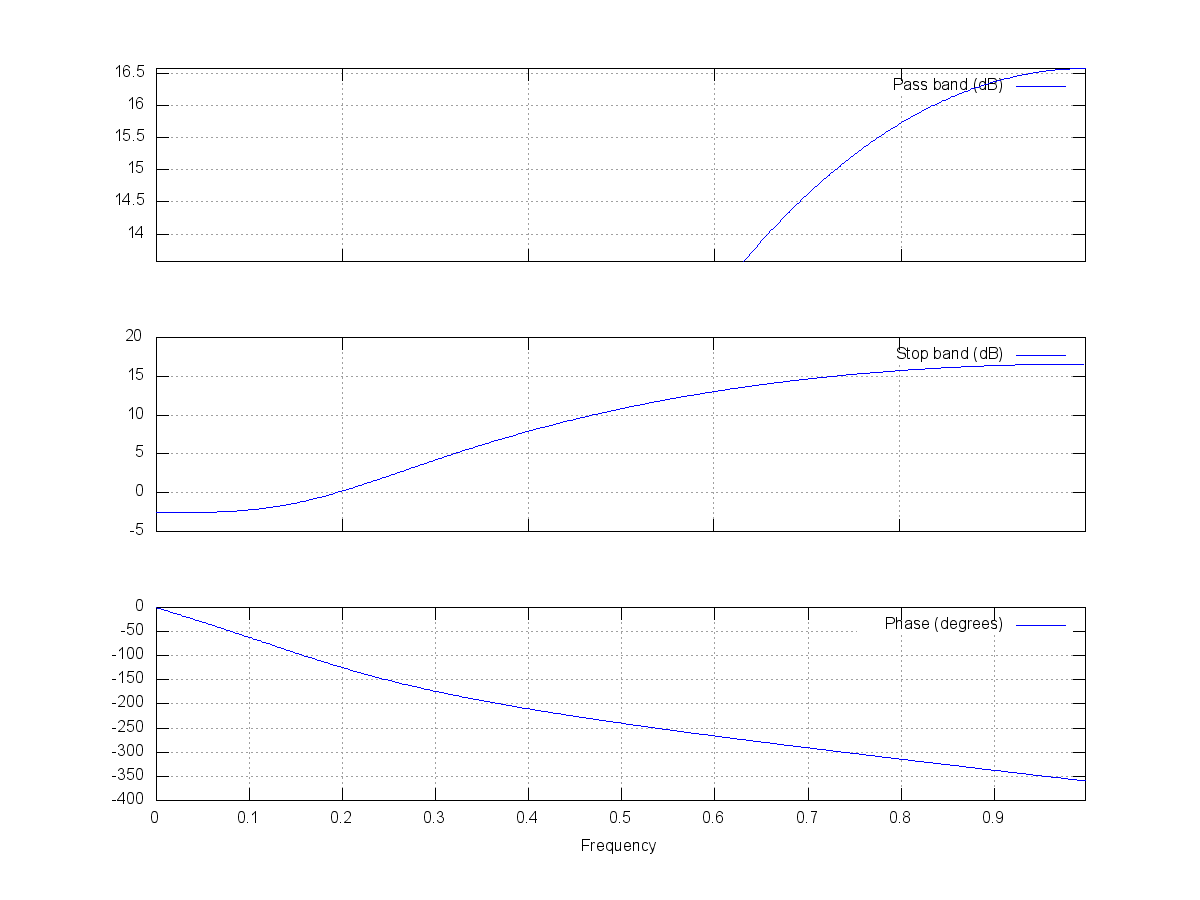
\includegraphics[scale=.3]{out/fig28.png}
      \caption{\label{fig28} Charakterystyka filtru, $b=1.5\pm0.7i$}

    \end{center}
  \end{figure}

  \begin{figure}[htbp]
    \begin{center}
      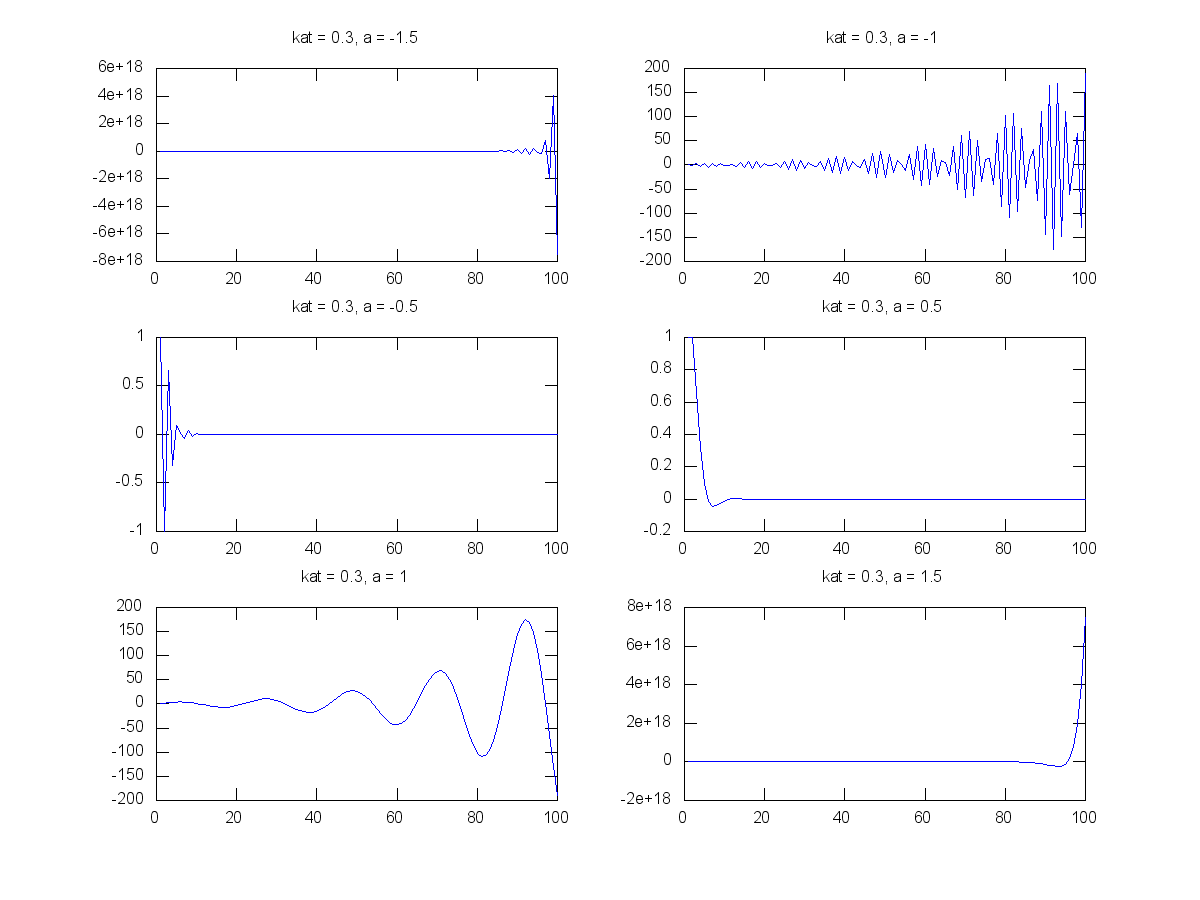
\includegraphics[scale=.3]{out/fig29.png}
      \caption{\label{fig29} Wpływ położenia zespolonego bieguna na odpowiedź impulsową (cz. 1)}
      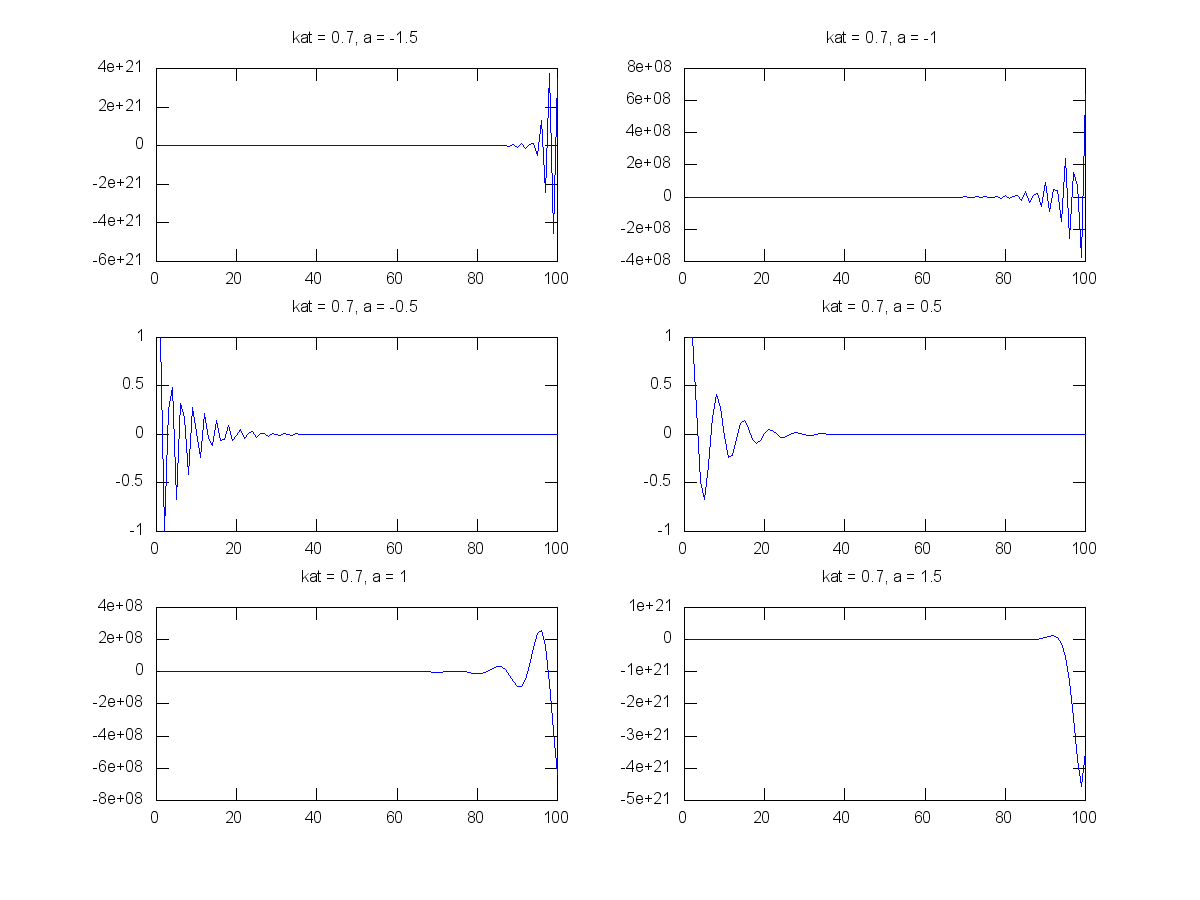
\includegraphics[scale=.3]{out/fig30.png}
      \caption{\label{fig30} Wpływ położenia zespolonego bieguna na odpowiedź impulsową (cz. 2)}

    \end{center}
  \end{figure}

  \begin{figure}[htbp]
    \begin{center}
      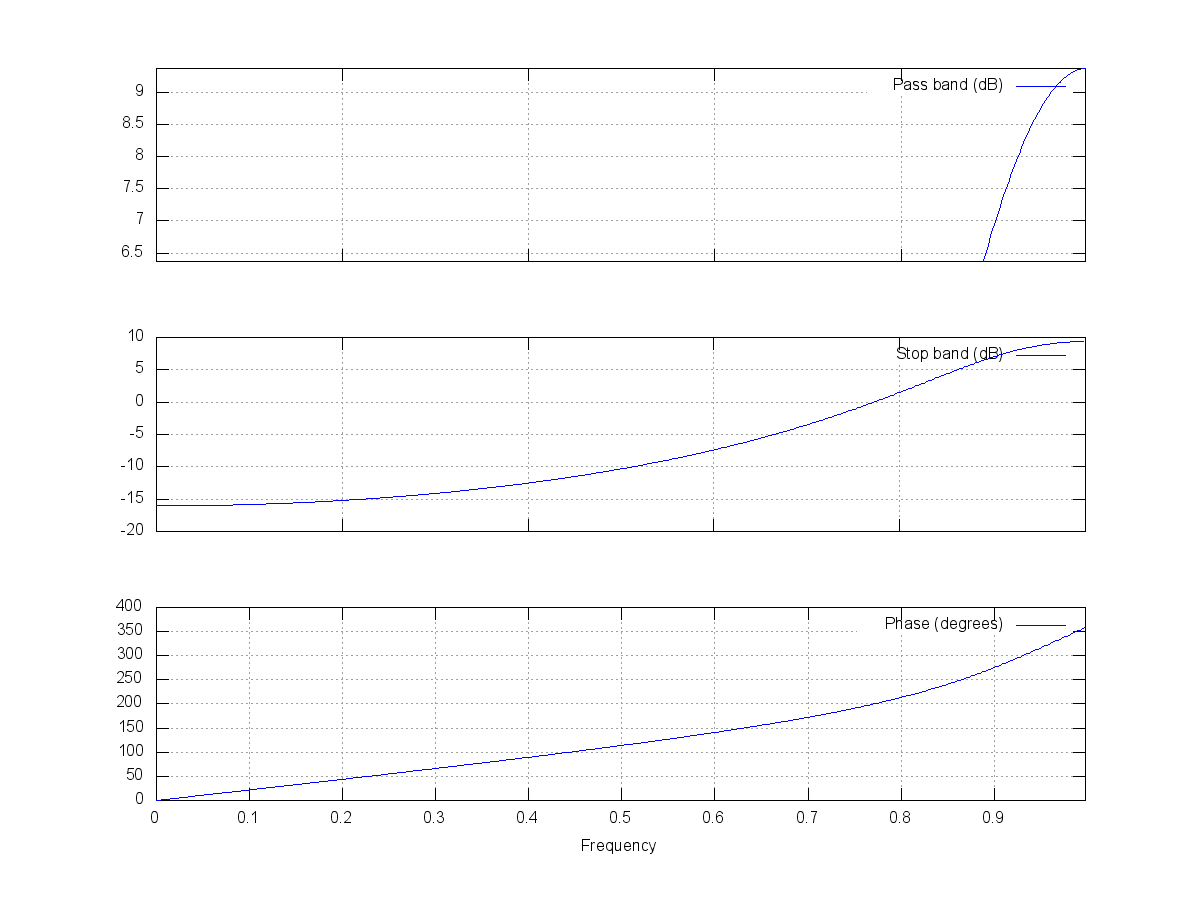
\includegraphics[scale=.3]{out/fig31.png}
      \caption{\label{fig31} Charakterystyka filtru, $a=-1.5\pm0.3i$}
      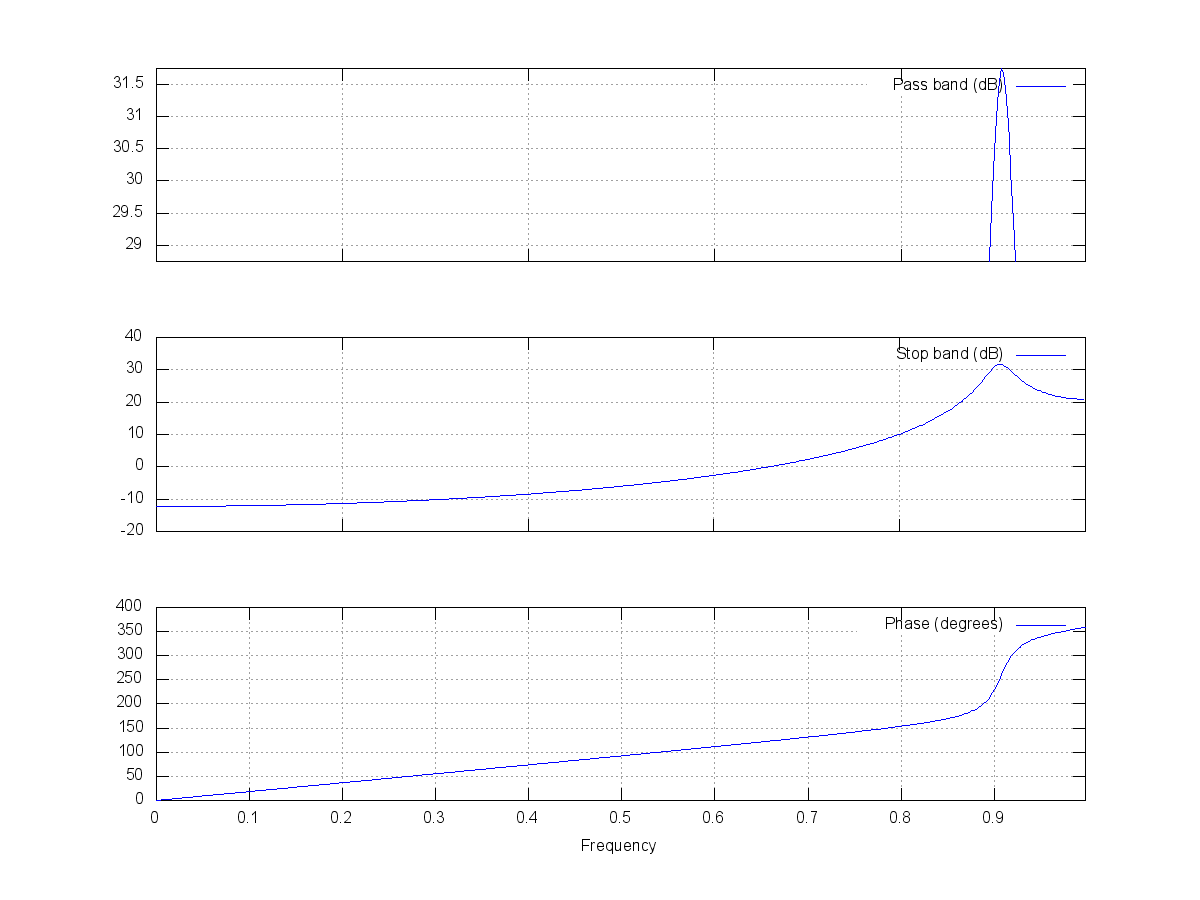
\includegraphics[scale=.3]{out/fig32.png}
      \caption{\label{fig32} Charakterystyka filtru, $a=-1.0\pm0.3i$}

    \end{center}
  \end{figure}

  \begin{figure}[htbp]
    \begin{center}
      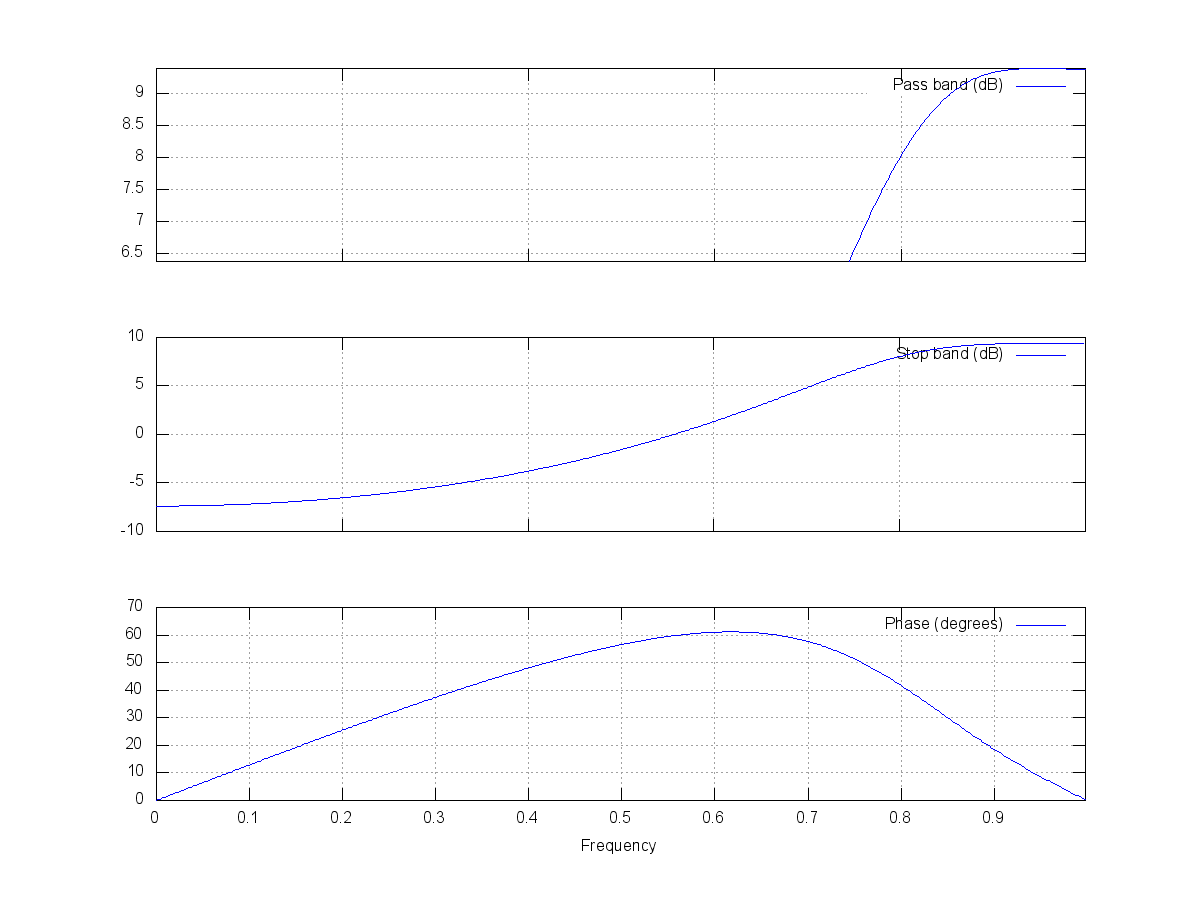
\includegraphics[scale=.3]{out/fig33.png}
      \caption{\label{fig33} Charakterystyka filtru, $a=-0.5\pm0.3i$}
      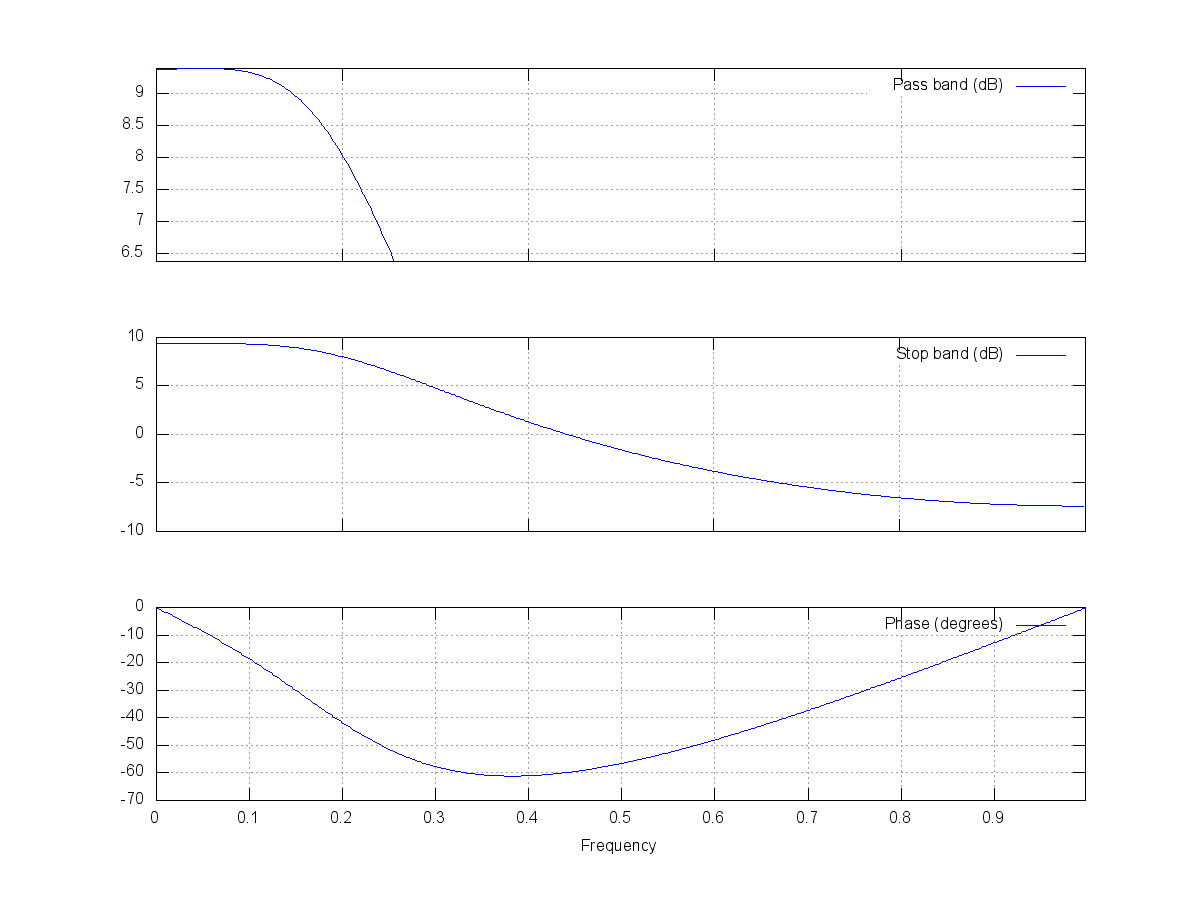
\includegraphics[scale=.3]{out/fig34.png}
      \caption{\label{fig34} Charakterystyka filtru, $a=0.5\pm0.3i$}

    \end{center}
  \end{figure}

\FloatBarrier

  \begin{figure}[htbp]
    \begin{center}
      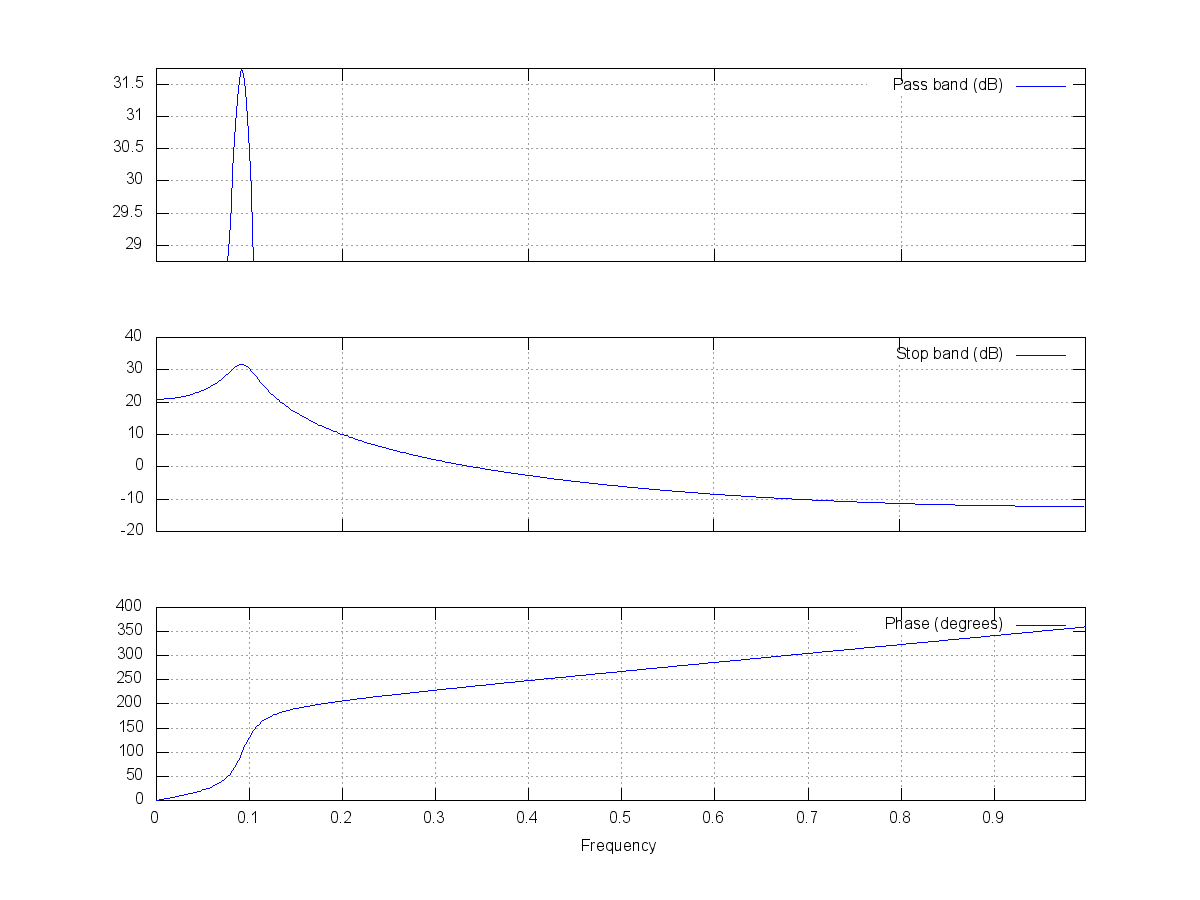
\includegraphics[scale=.3]{out/fig35.png}
      \caption{\label{fig35} Charakterystyka filtru, $a=1.0\pm0.3i$}
      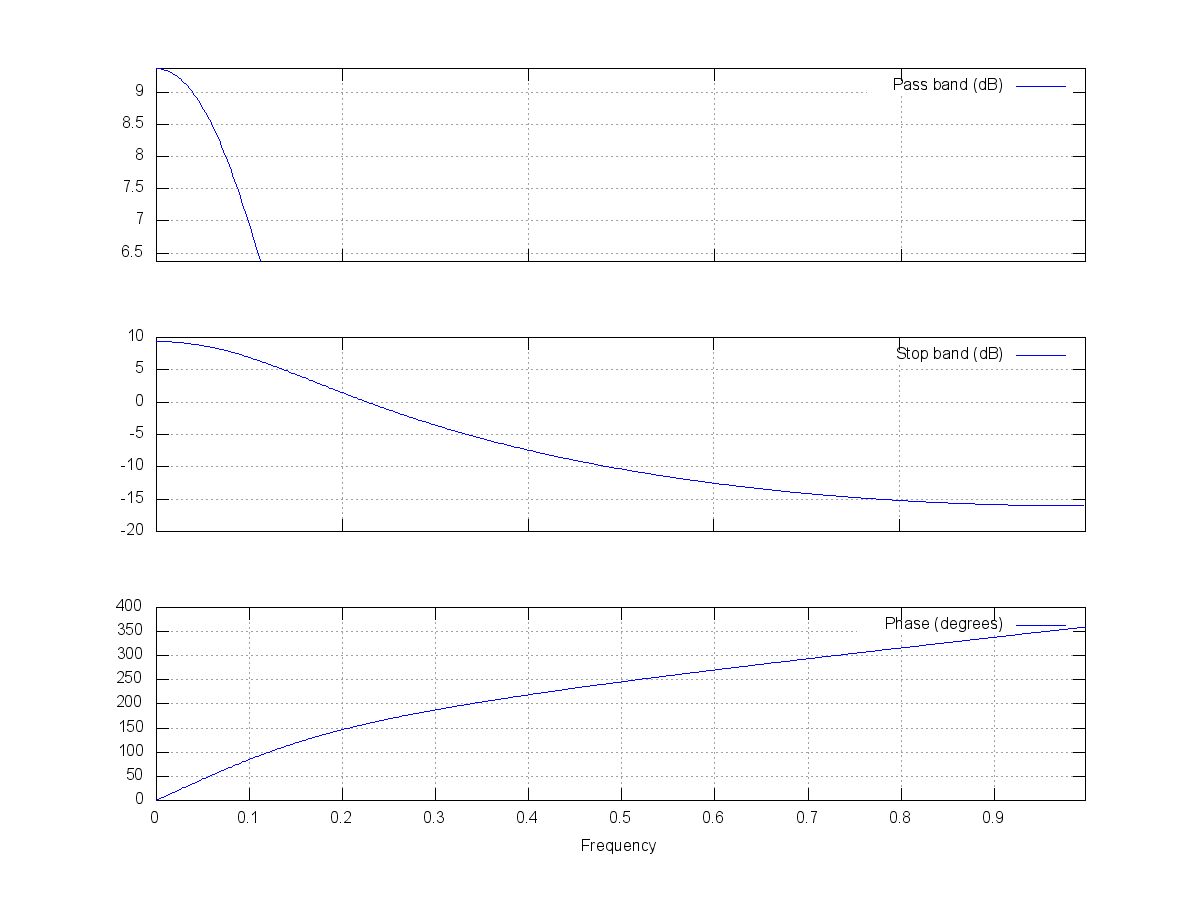
\includegraphics[scale=.3]{out/fig36.png}
      \caption{\label{fig36} Charakterystyka filtru, $a=1.5\pm0.3i$}

    \end{center}
  \end{figure}

  \begin{figure}[htbp]
    \begin{center}
      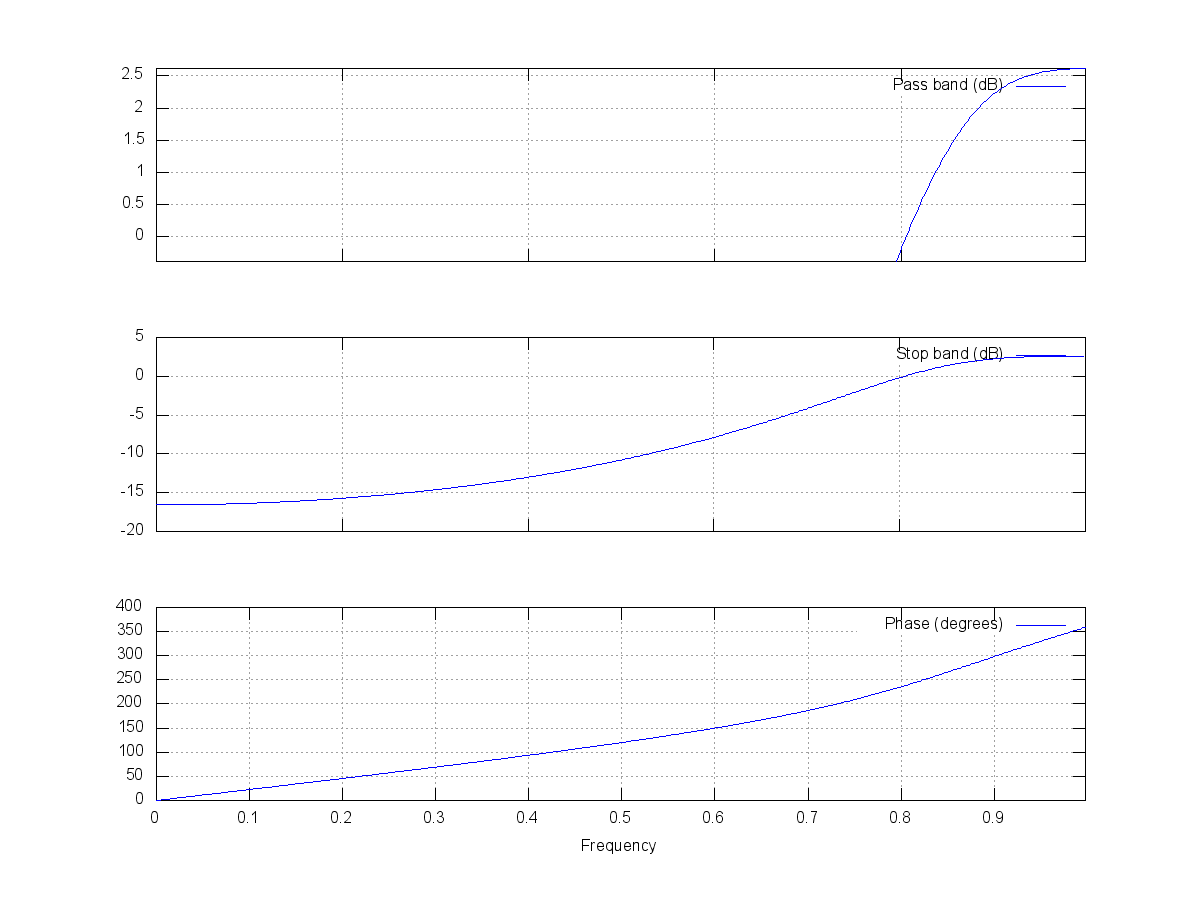
\includegraphics[scale=.3]{out/fig37.png}
      \caption{\label{fig37} Charakterystyka filtru, $a=-1.5\pm0.7i$}
      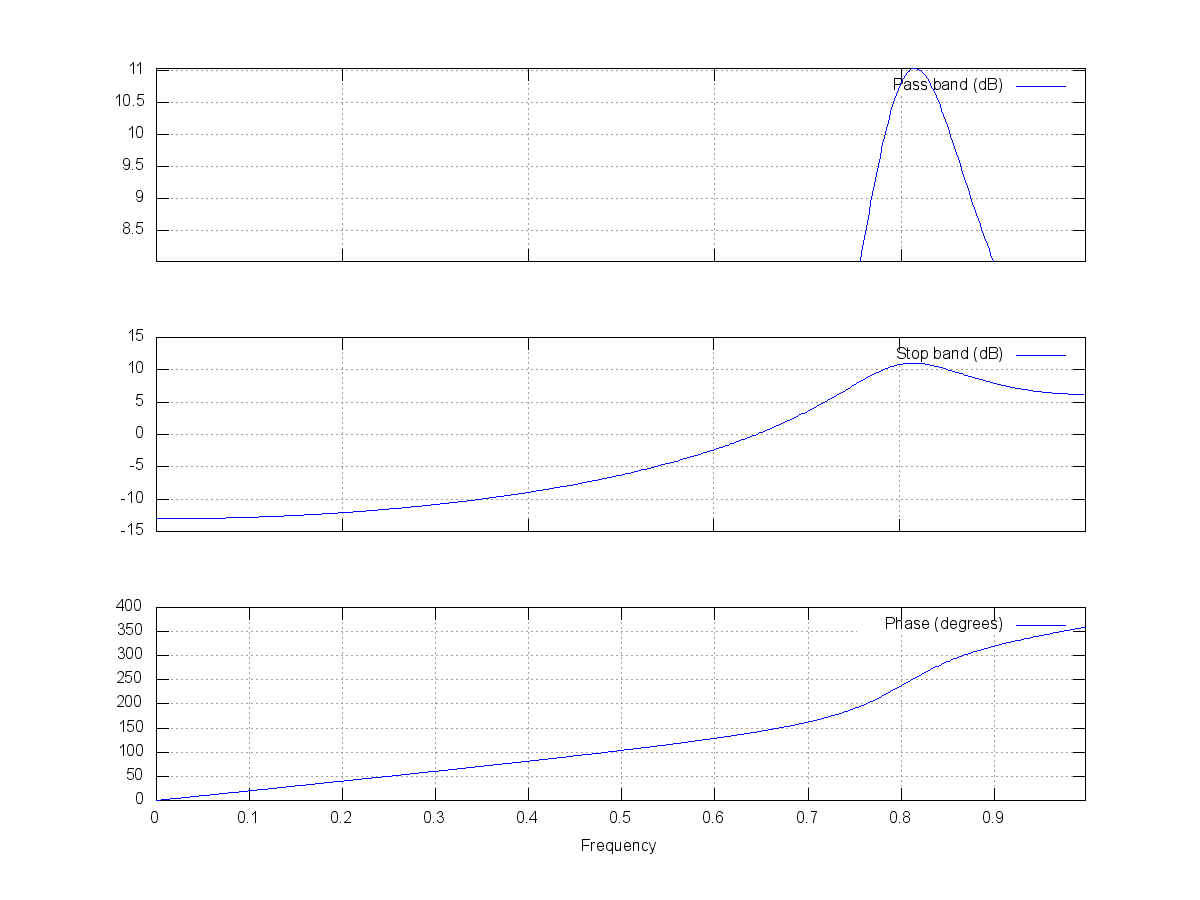
\includegraphics[scale=.3]{out/fig38.png}
      \caption{\label{fig38} Charakterystyka filtru, $a=-1.0\pm0.7i$}
  
    \end{center}
  \end{figure}

  \begin{figure}[htbp]
    \begin{center}
      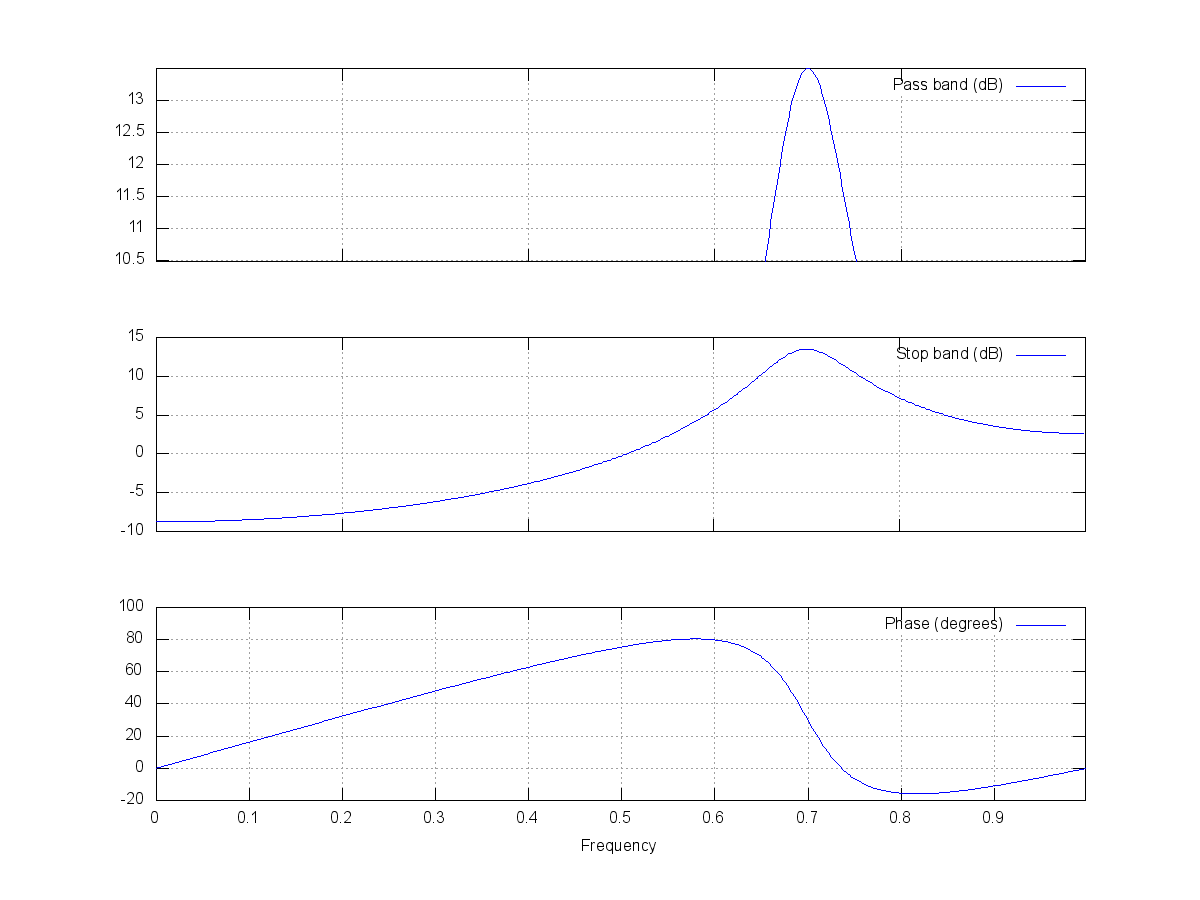
\includegraphics[scale=.3]{out/fig39.png}
      \caption{\label{fig39} Charakterystyka filtru, $a=-0.5\pm0.7i$}
      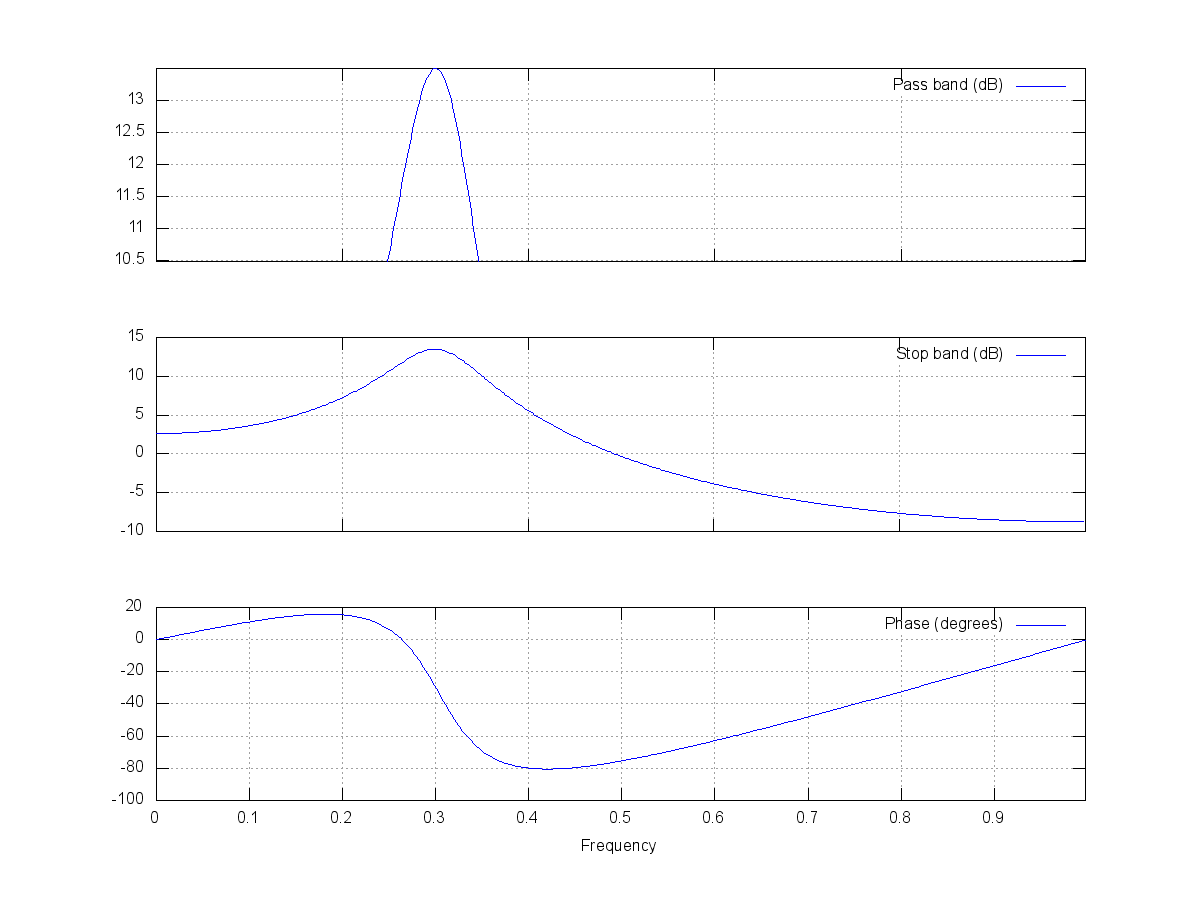
\includegraphics[scale=.3]{out/fig40.png}
      \caption{\label{fig40} Charakterystyka filtru, $a=0.5\pm0.7i$}
  
    \end{center}
  \end{figure}

  \begin{figure}[htbp]
    \begin{center}
      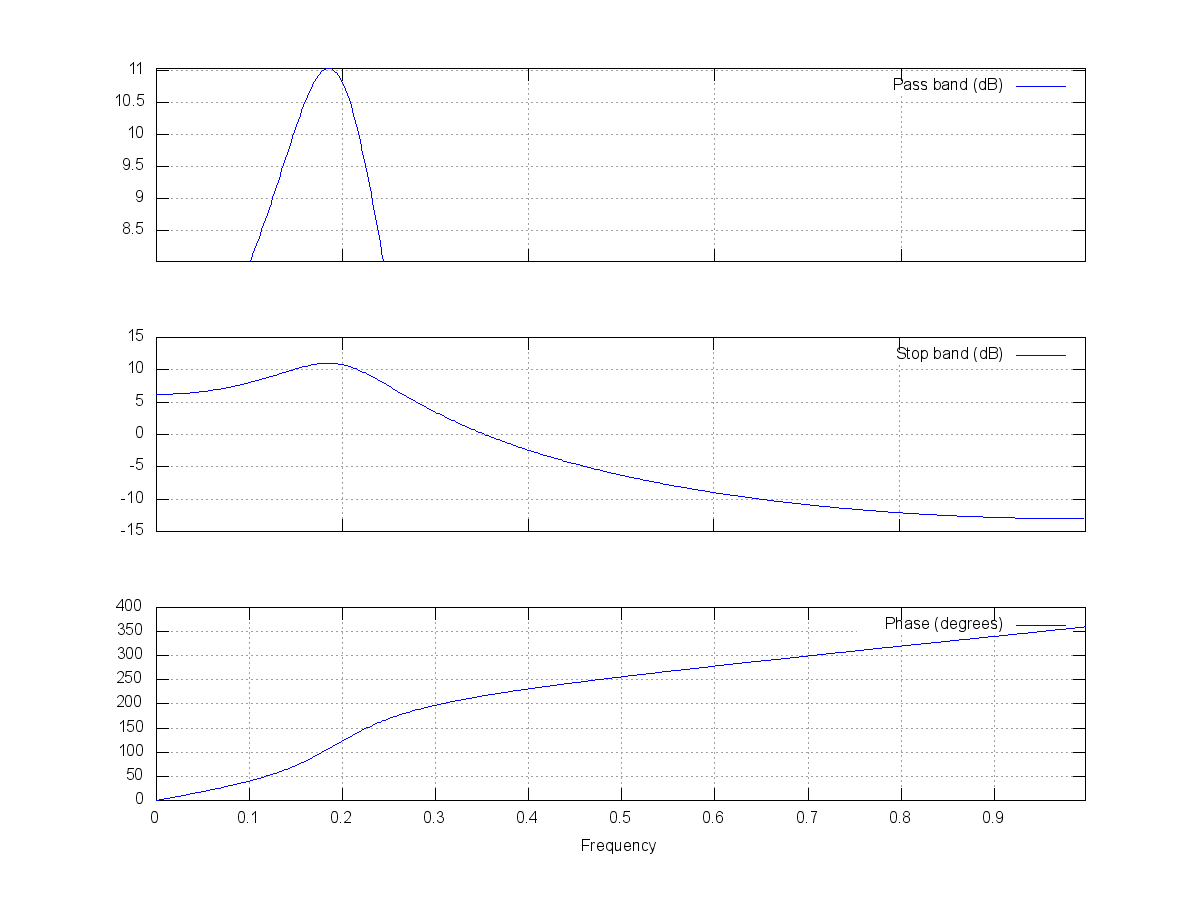
\includegraphics[scale=.3]{out/fig41.png}
      \caption{\label{fig41} Charakterystyka filtru, $a=1.0\pm0.7i$}
      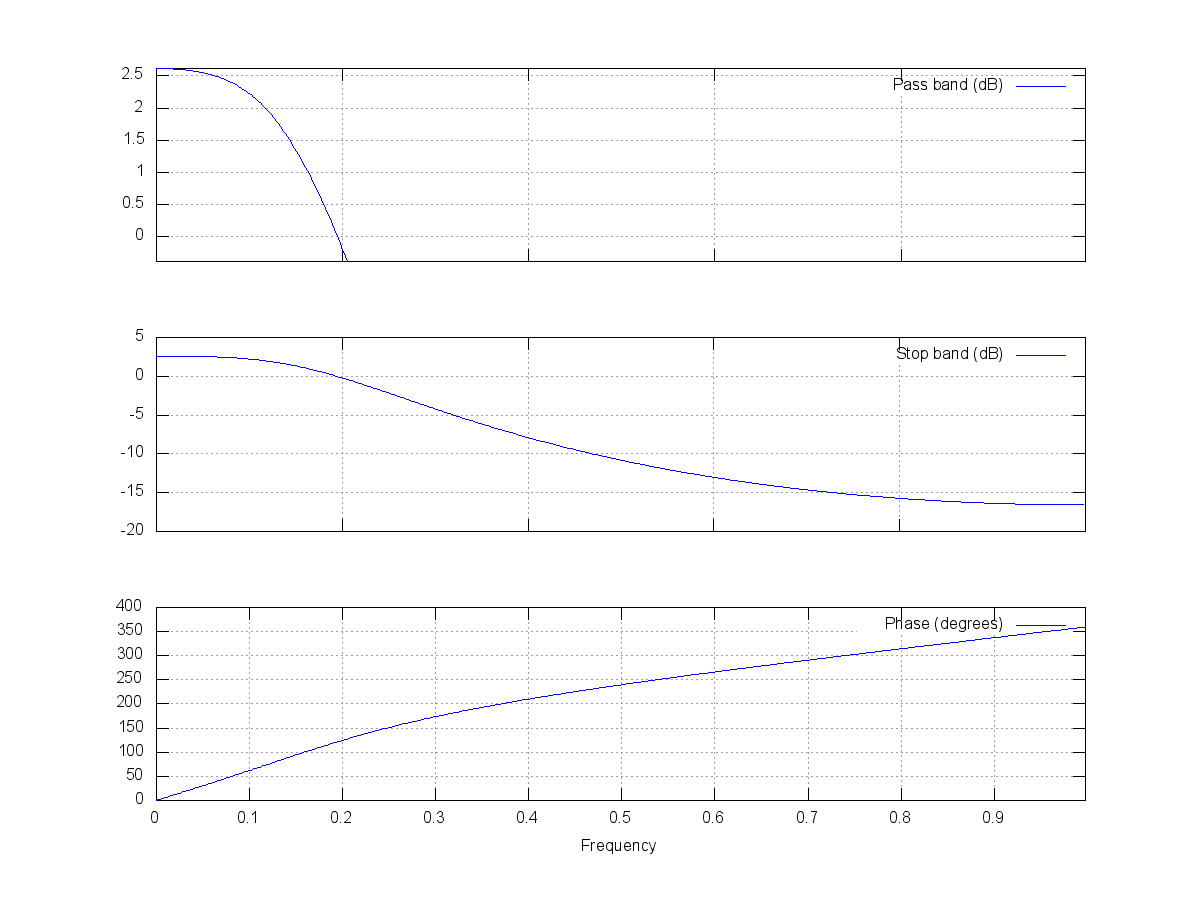
\includegraphics[scale=.3]{out/fig42.png}
      \caption{\label{fig42} Charakterystyka filtru, $a=1.5\pm0.7i$}
  
    \end{center}
  \end{figure}




\end{document}